\documentclass[a4paper]{report}

\usepackage[margin=1.5in]{geometry}

\usepackage [english]{babel}
\usepackage [autostyle, english = american]{csquotes}
\MakeOuterQuote{"}

\usepackage{hyperref}

\usepackage{graphicx}
\graphicspath{ {images/} }
\usepackage{dashrule}

% Maths packages
\usepackage{float}
\usepackage{amsmath}
\usepackage{amssymb}
\usepackage{enumitem}

\usepackage{booktabs} % For formal tables
\usepackage{mathtools}
\usepackage{tabu}
%\usepackage{arydshln}
\usepackage{nicefrac}

\DeclarePairedDelimiter\ceil{\lceil}{\rceil}
\DeclarePairedDelimiter\floor{\lfloor}{\rfloor}

\newcommand{\R}{\mathbb{R}}
\newcommand*\mean[1]{\bar{#1}}
\DeclareMathOperator*{\argmax}{arg\,max}

\usepackage {tikz}
\usetikzlibrary {positioning}

% Code snippet package setup
\usepackage{minted}
\definecolor{bg}{rgb}{0.95,0.95,0.95}

\usepackage{natbib}

% TODOs
\newcommand{\todo}[1]{\textcolor{red}{TODO: #1}\PackageWarning{TODO:}{#1!}}

\usepackage{array}
\newcolumntype{C}[1]{>{\centering}m{#1}}
\usepackage{tabularx}



\begin{document}
\title{\small Honours Thesis\\\huge Generating Clinical Queries from Patient Narratives}

\author{Liam Cripwell - 08857181\\liam.cripwell@connect.qut.edu.au\\\\\small Supervisor - Guido Zuccon\\\small g.zuccon@qut.edu.au\\}
\date{November 12, 2017}
\maketitle
\pagebreak

\begin{abstract}
This project investigates automated methods of formulating effective clinical search queries from verbose patient narratives. Currently, if a clinician is searching for medical documents to assist them in treating a patient, they must familiarise themselves with the patient's case, manually formulate a query and engage in the retrieval process themselves. Given a number of verbose patient narratives, a range of query reduction and expansion techniques were evaluated within the context of two separate document collections (biomedical literature and clinical trials). Comparison was made between a number of baselines, including full patient narratives and human generated queries. Query reduction proved to be an effective means of generating ad-hoc search queries from patient narratives; however, human generated queries were still significantly more effective than any automated reductions. Further improvements were possible if query reduction method parameter settings were determined on a per-query basis and a model for predicting this was developed. Under optimal conditions, pure reduction methods can exceed humans. Further significant improvement over automated reduction methods can be seen when pseudo-relevance feedback methods are applied. Future work should be directed towards investigating additional query reduction and expansion methods, as well as forming a more in-depth understanding of human query formulation in order to facilitate the further development of automated techniques.
\end{abstract}

\pagebreak
\tableofcontents
\pagebreak

\chapter{Introduction}
Clinical search is an area of Information Retrieval (IR) that investigates and develops methods of retrieval to assist with clinical tasks and decision making. The specific problem in question focuses on how the retrieval of clinical documents, such as medical literature and clinical trials, can be automated given a specific patient's medical record. Currently, clinicians must carry out such a retrieval task manually by first familiarising themselves with the patient record and then formulating what they believe to be an effective query with which they can retrieve these documents from a search engine. If effective automated methods can be developed, clinicians will be able to immediately view clinical documents related to a patient alongside the patient record, eliminating the need for them to personally invest time and effort into the retrieval task.

Existing work of a similar nature has been carried out within the TREC Clinical Decision Support (CDS) task \cite{Roberts2015Overview-of-the}. This task requires participants to develop retrieval methods that identify relevant medical literature while using verbose patient narratives as queries. These patient narratives act as substitutes for actual patient records and the high-level goal of the task is to identify medical literature that will effectively support the making of clinical decisions for the respective patient. Many query reformulation techniques were experimented with in this task, however the lack of a human benchmark makes it difficult to extrapolate how effective these automated techniques would be in a real life clinical setting, compared to clinician-formulated queries. 

A test collection containing human query benchmarks does exist for clinical trial documents \cite{Koopman2016A-Test-Collecti}. This collection makes use of the same patient narratives from the CDS collection, but for each narrative there exists a corresponding range of adhoc queries devised by clinicians. Initial work has been carried out with this test collection whereby a limited number of query reduction methods have been implemented and their retrieval performance evaluated in comparison to these human benchmarks. However, the methods tested in that work are rather limited in scope and leave a great deal of room for further investigation. The goal of this project is to expand upon the work done with the Clinical Trials collection~\cite{Koopman2016A-Test-Collecti} by investigating query reformulation techniques used in the context of the CDS task as well as more general approaches; all of which are examined in detail within Chapter 2.

\section{Research Process}

Initially, techniques to reduce the size of the patient narratives so that they form an effective query were investigated. Existing work carried out by CDS task participants were looked to here in order to determine which types of approaches performed well. In addition to this, more general query reduction techniques were examined. An important observation that was considered throughout this process was the fact that previous methods of reduction for verbose queries have only been used with significantly less verbose queries than the average patient narrative. Because of this, particular attention was paid to potential scaling issues arising from general reduction methods when applied to the narratives in their current form.

As was discovered in Koopman et al.~\cite{koopman2017generating}, the best performing human generated adhoc queries almost always consisted of novel terms (terms not explicitly existing within the narrative), which suggests that there may be an upper-bound on the level of performance possible by exclusively using reduction techniques. Because of this, there was a recognised need to investigate techniques that can be used to identify novel terms/concepts that are able to facilitate an improvement in retrieval performance. 

From this, our problem can be partitioned into two main areas: query reduction and query expansion. The project investigates these two topics via the following research questions:

\begin{itemize}
  \item \textit{Query Reduction}
    \begin{itemize}
      \item How can noisy terms be removed from the verbose query?
      \item To what extent can this improve retrieval effectiveness?
    \end{itemize}
  \item \textit{Query Expansion}
    \begin{itemize}
      \item Can external and implied information be used to improve retrieval effectiveness?
      \item What type of information proves valuable?
    \end{itemize}
\end{itemize}


\subsection{Query Reduction}
The first part of the project was focused on investigating query reduction techniques in order to develop a clearer understanding of the degree of retrieval performance that can be attained via pure reduction methods in comparison to human generated queries. Many different classes of reduction strategies were examined; some incorporating corpus statistics, some exploiting domain specific knowledge-bases, and others being primarily natural language processing and machine learning oriented. A range of techniques from the first two categories were implemented and evaluated, with some of the machine learning strategies used by the other techniques investigated being used to complement them.

\subsection{Query Expansion}
The next part of the project was focused on investigating methods that can potentially improve upon the automated reduction techniques examined during the earlier phase. This primarily involved the evaluation of various query expansion techniques that allow for the inference of novel terms into the formulated query, as well as document reranking methods in an attempt to improve the precision of retrieved documents. An investigation into post-retrieval document reranking techniques was also conducted. In particular, the biographical information and medical concept similarity based rerankers proposed by Soldaini et al.~\cite{SoldainiPlaceholder} were examined in detail as they are of particular interest within the context of our problem. This lead into an implementation of various pseudo-relevance feedback methods and an evaluation of their effect upon the retrieval effectiveness of existing reduction models. 

\section{Structure of Thesis}
This thesis will begin with a literature review exploring the existing body of work in the areas of automated query formulation (query reduction and expansion in particular), both generally and in the medical domain. Subsequently, the investigation and experiments conducted within this project will be addressed. The majority of this content is separated into main two components; one covering query reduction and the other covering query expansion. There is a logical division between these two components of the project and thus each section will contain its own experimental setup, results and discussion sections, before being drawn together and summarised towards the end of the report.


\chapter{Literature Review}
This chapter explores and reviews existing literature within the areas of query reduction and expansion. Reference is made to both general theory and applications, as well as those whose scope extends to within the medical domain or IR via patient records more specifically.

\section{Query Reduction}
One component of the query generation problem is that of \textit{reduction}. Sometimes queries can be rather verbose, acting as a verbalisation of the information need/context of the retrieval task. A verbose query generally does not perform as well as shorter queries that capture its most important features \cite{Balasubramanian:2010:ERL:1835449.1835545}. Query reduction involves reducing the size of a given query via a term pruning process. There are many different styles of approach taken here: some strategies involve reducing the number of terms in the query by using a statistical measure to determine importance of terms; some incorporate domain knowledge (often through the use of ontologies) in order to identify concepts that are likely important given the context and application domain of the search system; some utilise machine learning in order to identify important concepts within the query. 

Balasubramanian et al.~\citep{Balasubramanian:2010:ERL:1835449.1835545} provide a formal definition of the query reduction task to find the set $P^*$:

\begin{equation}
\begin{split}
P^* &= \argmax_{P\in \mathcal{P}^Q} T_f(P),
\end{split}
\end{equation}

where $Q$ is the original query, $\mathcal{P}^Q$ is the set of possible subqueries of $Q$, and $T_f$ is the measure of retrieval effectiveness for a given query. However, because it is not viable to calculate $T_f$ for every $P$, estimations must be made; this gives us the revised definition of $P^*$:

\begin{equation}
\label{QRdefinition-lit}
\begin{split}
P^* &= \argmax_{P\in \mathcal{P}^Q} \widehat{T_f}(P)
\end{split}
\end{equation}

The query reduction task thus becomes the problem of finding an effective method of estimating values of $T_f$ in order to produce the best possible value of $P^*$. This section explores existing work conducted in this area.

\subsection{Methods Based On Collection Statistics}

One class of query reduction techniques are those that use some collection-derived statistical measure(s) in order to rank the query terms and subsequently construct a new query with a subset of the most highly ranked terms. One measure commonly used throughout the field of information retrieval is Inverse Document Frequency (idf). This is used as a measure of a term's importance throughout the document collection. The idf of a particular term $t$ is calculated as follows:

$$idf_t = \log{\frac{1+N}{df_t}}$$

where $N$ is the total number of documents in the collection and $df_t$ is the document frequency of $t$ (number of documents in collection that contain $t$).

This method was analysed by Koopman et al.~\citep{koopman2017generating} in the contex of deriving effective search queries from verbose patient narratives by reducing the narrative to a subset of terms with the highest ranking idf values. They used a proportion-based pruning method whereby some reduction parameter $r$ in the range [0,1] is used to determine the percentage of original terms that are retained throughout the reduction process. Formally, a reduction resulting from this method can be seen as comprising of the terms in the following set:

$$Q' = \{ t : s(t,Q) \leq |Q| \cdot r \}$$

where $s(t,Q)$ is the ranked position of term $t$ within query $Q$ based on its idf score, $|Q|$ is the number of terms in the original query, and $r$ is the retention percentage.

The results of that work show that when an appropriate value of $r$ is used a statistically significant increase in retrieval effectiveness can be seen when compared to the case of the patient narrative in its entirety being used as the query. Although this reveals that the removal of less informative terms from a verbose patient narrative is a simple way to improve retrieval effectiveness, the method's reliance on an appropriate value of $r$ severely cripples its ability to adapt optimally to a wide range of narratives without the incorporation of some additional predictive component. This raises the further question of how such a value for $r$ could be estimated.

\subsection{Methods Based On Query Performance Prediction}

Another class of query reduction strategies explored in previous work are those that aim to formulate some predictive framework within which the performance of a given query can be estimated ahead of time. Formally, this aim is to estimate the value of $\widehat{T_f}(P)$, as defined in Equation \ref{QRdefinition-lit}. Sub-queries of the original verbose query are then subjected to this framework in order to find the alternative with the greatest predicted level of performance. Methods of predicting the performance of a query, known as \textit{query performance prediction} (QPP), have previously been investigated within studies seeking to improve IR system robustness (ability to handle poor-performing queries)~\cite{HE2006585}. Having the ability to estimate the performance of a query either before or at retrieval time allows a system to take action to hopefully improve the eventuating retrieval effectiveness. A general approach to this problem is to use various \textit{pre-retrieval predictors}, derived from query terms, collection statistics and relevant external sources, in order to formulate an estimated degree of performance without having to actually engage in the computationally intensive retrieval process \cite{Hauff:2008:SPQ:1458082.1458311}. 

QPP techniques have been utilised quite extensively within the area of query reduction. One such application is that of Kumaran and Carvalho~\citep{Kumaran2009Reducing-Long-Q} who approached the query reduction problem by generating shorter subqueries from the initial query and training a classifier to predict the quality of a given subquery based on various predictive measures. The measures used by Kumaran and Carvalho are as follows:

\textbf{Subquery Length (SQLen)}:
Number of terms in the subquery.

\textbf{ Mutual Information (MI)}:
A graph is constructed by calculating the MI between every subquery term and assigning these as edge weights. A value is then determined by identifying the maximum spanning tree and averaging it's edge weights. Mutual Information is computed as:
$$MI(x,y) = \log \frac{\frac{n(x,y)}{T}}{\frac{n(x)}{T}\frac{n(y)}{T}},$$
where $n(x)$ and $n(y)$ are the number of documents containing terms $x$ and $y$ respectively, $n(x,y)$ is the number of documents containing both terms, and $T$ is the total number of terms in the collection.

\textbf{Query Clarity (QC)}:
The Kullback-Leibler divergence of the query model from the collection model. The query model is estimated from the top-ranked documents retrieved by the original query. 
$$QC = \sum_{w\in Q} P(w|Q) \times \log_2{\frac{P(w|Q)}{P_C(w)}},$$ where $P(w|Q)$ is the probability of the occurence of the word $w$ in the query model, and $P_C(w)$ is the probability of the occurrence of $w$ in the collection.


\textbf{Simplified Clarity Score (SCS)}:
$$SCS = \sum_{w\in Q} P_{ml}(w|Q) \times \log_2{\frac{P_{ml}(w|Q)}{P_C(w)}},$$ 
where $P_{ml}(w|Q)$ is the probability of the occurrence of the word $w$ in the query, using the maximum likelihood estimation.

\textbf{IDF-based features}:
sum; standard deviation; maximum/minimum; arithmetic mean; geometric mean; harmonic mean; and coefficient of variation.

\textbf{Query Scope (QS)}:
A measure of the size of the retrieved document set relative to the collection size:
$$QS = -\log{\frac{n_Q}{N}},$$ 
where $n_Q$ is the number of documents that contain at least one of the query terms.

\textbf{Similarity Collection/Query-based features (SCQ)}:
A measure of how similar a query was to the collection as a whole; averaged across all query terms.
$$SCQ_w = (1+ \ln{\frac{n(w)}{N}}) \times \ln{(1 + \frac{N}{N_w})},$$
where $N_w$ is the document frequency of $w$, and $n(w)$ is the collection frequency of $w$. 

\textbf{Inverse Collection Term Frequency (ICTF)}:
$$ICTF_w = \log_2{\frac{n(w)}{T}},$$
where $T$ is the total number of terms in the collection.

\textbf{Similarity Original Query (SOQ)}:
The cosine similarity between the tf*idf vectors representing a subquery and the original query.

A ranking function is then generated with each of these measures as a feature via a learning-to-rank algorithm (RankSVM in that particular study). Once an effective ranking function exists, these predictors are calculated for each possible subquery of a given query and the candidate with the highest predicted performance is selected as the reduced query.

This technique does not translate smoothly to our problem, given the difference in the degree of verbosity exhibited by our initial queries. Our patient narratives are significantly larger than those used within the study of Kumaran and Carvalho, and as a result many of the statistics used require far too much computational effort. In addition, generating permutations of subqueries becomes a factorially more expensive task that enters the realm of complete infeasibility within the context of our problem. For example, a query with 5 terms would have $5!$ (120) possible subqueries, whereas a query with 200 terms (actual size of some patient narratives) would have $200!$. Even when subqueries are generated as permutations of noun phrases, the level of computation to be computed at runtime for some of these query predictors is extreme \cite{koopman2017generating}.

Soldaini et al. attempt to reduce the computational load of this task with their \textit{FastQQP} method~\cite{Soldaini2015RetrievingML}. The authors propose a revised approach to QPP candidate selection that prunes the range of candidate subqueries as early in the computational process as possible in order to reduce the total time and complexity involved. This is done by first calculating the Mutual Information score for each candidate subquery and pruning the set so that it is comprised of only the top-$k$ candidates for each possible candidate query length. The remaining QPP measures are then calculated for the resulting set of candidates. 

Although this modified approach may drastically reduce the computational complexity involved in the process, it is still not insignificant. In Koopman et al.~\cite{koopman2017generating} merely calculating the Mutual Information score for all candidate subqueries of particularly verbose patient narratives proved to be infeasible. Perhaps further enhancing the \textit{FastQQP} approach with a more aggressive pruning criteria or substituting Mutual Information for a measure of less computational complexity could result in a query performance prediction technique that proves feasible within the context of verbose patient narratives; or particularly verbose queries in general.

Balasubramanian et al.~\citep{Balasubramanian:2010:ERL:1835449.1835545} explored various reduction techniques for verbose web queries that employ the use of query performance prediction. The authors presented a range of different learning formulations that utilise different combinations of predictors and weighting strategies in order to effectively choose a reduced subquery. They acknowledge the infeasibility of evaluating every potential subquery of a given query and propose an alternative approach by which only those subqueries that differ from the original by a single term are evaluated. Part of their rationale behind such an assumptive stance when it comes to reducing the size of the candidate set is the inherent importance of fast response times that exists within the web search domain. 

However, such an alternative approach is unlikely to successfully translate to our problem given the paper is concerned with long \textit{web} queries, which are presumably of a much shorter length than the patient narratives. More concretely, when Koopman et al.~\citep{koopman2017generating} investigated statistical reduction methods with the same collection of patient narratives we use here, it was found that retrieval effectiveness peaked when the narrative was reduced to approximately 25-30\% of its original size. Despite this hypothesised incompatibility, a candidate set reduction of a similar nature could be included as part of a combined reduction method, whereby the narrative would already be reduced substantially or converted to an alternative representation (e.g. set of noun-phrases; cf. bag-of-words). 

\subsection{Methods Based On Domain Knowledge}

A common approach to verbose query reduction in the medical domain is to identify medical concepts present within the query and create a new query consisting of just these concepts. This approach was taken by Soldaini et al.~\citep{Soldaini2015RetrievingML} whereby the UMLS medical ontology was used to identify medical concepts and subsequently the query was reformulated to only include those terms that had a mapping to a concept within the system. The same approach was taken by Koopman et al.~\citep{koopman2017generating} in the context of using patient narratives to search for clinical trials. The results of this study showed that simply removing non-medical terms from a narrative produces very good retrieval results. The pure UMLS reduction method also produced better results than an idf reduction method, which was also tested in the same retrieval task by Koopman et al.
  
A similar method was also investigated by Soldaini et al.~\cite{Soldaini2015RetrievingML} whereby queries were reduced to contain only \textit{health-related} terms, as opposed to explicit medical concepts. This was achieved by obtaining a Wikipedia dump consisting of 2.7 million pages and classifying each as being "medically related" if they contained $\geq 1$ medical concepts. For each term candidate $c_l$ in the original query, they estimated its likelihood of being associated with a health related Wikipedia entry by comparing the odds ratio between the probability of an entry $P$ being health related when $c_l \in P$ over the probability of $P$ not being health related over all Wikipedia entries: 

\begin{equation}
\label{hrterms-lit}
\begin{split}
OR(c_l) &= \frac{Pr\{ P \text{ is health-related } | c_l \in P\}}{Pr\{ P \text{ is not health-related } | c_l \in P\}}
\end{split}
\end{equation}

A term is retained as part of the generated reduction if $OR(c_l) \geq \delta$, where $\delta$ is a tuning parameter; the optimal value of which was empirically determined to be 2.

This approach differs from the pure UMLS reduction approach as it allows for the retention of terms which, although not forming part of a medical concept themselves, could still be important within the structure of a medically-oriented query. This approach produced significantly better retrieval results to that of the UMLS reduction approach within the context of the problem ~\citep{Soldaini2015RetrievingML}. The authors themselves submitted that this is likely a product of the less aggressive reduction strategy of the health-related term reduction model. These findings suggest that it would be valuable to implement a variant of this technique within the context of our own task.
  
Koopman et al.~\cite{Koopman2011AEHRC--QUT-at-T} experimented with a concept-based information retrieval approach to medical record search. Here, all queries as well as documents were converted from their term-based representations into a "bag-of-concepts" representation by identifying all UMLS concepts existing within the content of each. This differs from the approach taken in Soldaini~\citep{Soldaini2015RetrievingML} and Koopman et al.~\citep{koopman2017generating} as the concept identification itself becomes a part of the query as opposed to the terms that form a part of a concept being retained. In this way, the ambiguity imported into the problem by synonymous concepts is removed. 

Limsopthan et al.~\citep{Limsopatham2013A-Task-Specific} took a very similar approach to the pure UMLS reduction method, however applied a more aggressive pruning criteria by retaining only those medical concepts that were identified as being a symptom, diagnostic test, diagnosis, or treatment concept. The motivation behind this decision is that these four types of medical concepts are the most commonly considered by health practitioners when dealing with patients \cite{Ely429}. Koopman et al.~\citep{koopman2017generating} tested a variant of this approach whereby UMLS concepts classed as either diagnosis, test, or treatment related terms were retained to form the reduced query. The retrieval results produced by this method proved to be rather poor; showing very minor increase in performance when compared to using the entire verbose narrative itself.


\subsection{Methods Based On Classification/Learning}

Many state-of-the-art query reduction techniques leverage machine learning in order to reliably construct and select subqueries that will improve retrieval performance. These often rely on term classification methods that prune the total set of query terms by labelling each as either useful or not useful. This section explores a number of well known techniques in this area.
  
Bendersky and Croft~\cite{Bendersky:2008:DKC:1390334.1390419} developed a technique for automatically extracting key concepts from verbose queries that have the most impact on retrieval effectiveness. They approach this by using various features in order to identify and weight concepts that exist within a query and subsequently generate a revised reduction from these concepts through the use of a probabilistic model. The technique aims to rank each given document, $d$, in response to a given query, $q$, by estimating the probability $p(q|d)$. This is achieved by considering all concepts within $q$

\begin{equation}
\label{one}
\begin{split}
p(q|d) &= \sum_{i}{p(q|d,c_i)p(c_i|d)},
\end{split}
\end{equation}

where $c_i$ is a given concept. From this, linear interpolation of $p(q|d)$ and $p(q|c_i)$ can be used to estimate $p(q|d,c_i)$. From this, a document ranking estimation function is formed:

$$rank(d) = \lambda' p(q|d) + (1-\lambda') \sum_{i}{p(q|c_i)p(c_i|d)},$$

where $\lambda'$ is a free parameter in the range [0,1]. Assuming a uniform distribution for both $p(q)$ and $p(c_i)$, and that only concepts explicitly within the query are used, this function is rank-equivalent to the following:

\begin{equation}
\label{2}
\begin{split}
rank(d) \propto \lambda p(q|d) + (1-\lambda) \sum_{c_i \in q}{p(c_i|q)p(c_i|d)},
\end{split}
\end{equation}

where $\lambda$ is normalised such that $\lambda = \frac{\lambda'}{\lambda' + \frac{p(q)}{p(c_i)} (1-\lambda')}$. This equation is used to determine the degree of benefit to performance contributed by concept identification and weighting.

The authors used noun-phrases existing within the query as concepts. The consideration of noun-phrases as query concepts has been proven to be reliable in existing work \cite{Xu:1996:QEU:243199.243202}. Given Equation \ref{2}, $p(c_i | q)$ is treated as a weighting assigned to each query concept to reflect how representative of the original query it is. In order to evaluate this weighting, the following assumptions are made:

\begin{enumerate}
  \item Each concept $c_i$ can be assigned to one of the two classes:
    \begin{itemize}
      \item KC - \textit{Key Concept}
      \item NKC - \textit{Non-Key Concept}
    \end{itemize}
  \item A global function $h_k(c_i)$ exists, which indicates the "confidence" of $c_i$ being within the KC class.
\end{enumerate}

Given these two assumptions, a normalized variant of $h_k(c_i)$ is used to derive an estimate:
\begin{equation}
\label{kcestimate}
\begin{split}
\hat{p}(c_i|q) &= \frac{h_k(c_i)}{\sum_{c_i \in q}{h_k(c_i)}}
\end{split}
\end{equation}

This works to the effect that the concepts with the highest \textit{confidence} are regarded as the best representations of the query. In order to deduce $h_k(c_i)$, a supervised machine learning approach is used. Different weighting measures are calculated and used as the input features for the weight assignment algorithm. A training set of labelled instances can be considered as follows:
$$(\chi_1,l_1), ..., (x_n,l_n),$$
where $x_i$ is a feature vector representing concept $c_i$, and $l_i$ is a binary label of whether or not $c_i \in KC$. Given the training set, an attempt is made to learn a ranking function of the form $h_k: x \rightarrow \R$. Once the learning phase is carried out, $h_k(c_i)$ is used to estimate a value for $\hat{p}(c_i|q)$, via Equation \ref{kcestimate}. The weighting measures seen in Table \ref{kc-features} are used as features in the learning method.

\begin{table}
\caption{Key Concepts learning features}
\begin{center}
  \begin{tabular}{ | c | l | }
  	\hline
    \textbf{Feature} & \textbf{Description}\\
    \hline 
    $is\_cap(c_i)$ & Boolean indication of whether all words are capitalised. \\
    $tf(c_i)$ & Collection term frequency. \\
    $idf(c_i)$ & Inverse document frequency. \\
    $ridf(c_i)$ & Residual inverse document frequency. \\
    $wig(c_i)$ & Weighted information gain. \\
    $g\_tf(c_i)$ & Term frequency extracted from Google n-grams counts. \\
    $qp(c_i)$ & Number of times concept formed a part of a query (extracted from a query log). \\
    $qe(c_i)$ & Number of times concept was used as a query (extracted from a query log). \\
    \hline
  \end{tabular}
\end{center}
\label{kc-features}
\end{table}

Results from an analysis of feature performance suggest that smaller corpora should use features other than collection, term and document counts in order to prevent concept frequency underestimation. This should be taken into consideration for our problem as our corpus is relatively small (in comparison to those investigated within the study in question). However, as we do not have access to query logs, some focus should be applied to the task of choosing effective features. Perhaps an alternative to query log features could be devised via examining the collection of patient narratives and ad-hoc queries. It remains to be seen whether this will be of any benefit considering the small set size. 

Three different document collections were used throughout Bendersky's investigation: ROBUST04 (a newswire collection), W10g and GOV2 (both web collections). 

\begin{table}
\caption{Document collection statistics}
\begin{center}
  \begin{tabular}{ | c | c | c | }
  	\hline
    \textbf{Name} & \textbf{\# Docs} & \textbf{Query Lengths}\\
    \hline 
    ROBUST04 & 528,155 & - \\
    W10g & 1,692,096 & - \\
    GOV2 & 25,205,179 & - \\
    ClinicalTrials & 204,855 & 39-204 \\
    \hline
  \end{tabular}
\end{center}
\end{table}

Multiple key concepts were more common in the ROBUST04 collection than the other two collections as its topics tend to contain more verbose and grammatically complex description queries. This may provide some degree of explanation for a notably lower classification accuracy exhibited against the ROBUST04 collection compared to the others. This observation could extend to within the scope of our problem, as the level of verbosity exhibited by the patient records may share some classification accuracy diminishing qualities with those of the ROBUST04 collection. 

It was found that adding more than two concepts attains no further increase in performance gain. Again, it is worth noting that this may be different when applied to patient records as they are generally much greater in length than the queries used in this study (39-204 terms in length compared to 12-49). The nature of patient narratives being an overview of an individual's entire medical profile suggests a need for a larger number of concepts in order to accurately capture relevant documents within their retrieval scope. Overall, the retrieval results of the experiment showed that the key concept reduction model outperforms the original queries to a statistically significant degree, and has comparable performance to that of a more elaborate and computationally intensive model which was tested alongside it (sequential dependency model). 
  
Xue et al.~\cite{Xue:2010:IVQ:1871437.1871572} outline an approach that frames subquery selection as a sequential labelling problem whereby each query term is processed and labelled with "keep" or "don't keep".  They propose that relationships between query terms imply a relationship between their assigned labels and therefore, subquery selection is more appropriately performed via sequential labelling rather than classifying the query terms in isolation. In order to do this, they make use of a task-specific variant of a Conditional Random Field (CRF) graphical model, which generates the distribution of subqueries while capturing the local and global dependencies existing between the query terms.

Three different types of features are used in their model to capture the concept/term dependencies existing within the queries. 

\begin{itemize}
  \item Independency Features
    \begin{itemize}
      \item Basic features of single query terms such as corpus/document frequencies, etc.
    \end{itemize}
  \item Local Dependency Features
    \begin{itemize}
      \item Used to capture dependencies between query terms. These includes bigrams, named entities, noun phrases and subject/object relationships.
    \end{itemize}
  \item Global Dependency Features
    \begin{itemize}
      \item Used to describe properties of the query as a whole. Many of the global dependency features used in this study are the same predictors used by Kumaran and Carvalho's QPP technique \cite{Kumaran2009Reducing-Long-Q}. 
    \end{itemize}
\end{itemize}

The authors attempt to train a subquery selection model given an original query and its entire set of subqueries, along with each of their retrieval performances. This immediately raises red flags in terms of performance issues given our particular problem, as it has already been noted that subquery generation for verbose patient narratives is a very computationally intensive task \citep{koopman2017generating}. However, as has been raised earlier, if a method of mitigation for this problem is devised (whether it be a pre-reduction step, an alternative to term-based pruning, etc.) then the viability of this can be reconsidered.

Their novel CRF is able to be trained with a combination of different retrieval models and performance measures. In their paper they experiment with four retrieval models, some using just the selected subquery, some with a combination of the subquery and the original query.

\textbf{SubQL:}
\begin{equation}
\begin{split}
  score_{QL}(D, Q_s) &= \sum_{t \in T(Q_s)} \log(P(t|D))
\end{split}
\end{equation}

where $T(Q_s)$ is the term set of subquery $Q_s$ and $P(t|D)$ is the probability of generating term $t$ from document $D$.

\textbf{SubDM:}
\begin{equation}
\begin{split}
  score_{DM}(D, Q_s) &= \lambda_T \sum_{t \in T(Q_s)} \log(P(t|D)) \\
  + \lambda_O \sum_{o \in O(Q_s)} \log(P(o|D)) &+ \lambda_U \sum_{u \in U(Q_s)} \log(P(u|D))
\end{split}
\end{equation}

where $O(Q_s)$ is the set of ordered bigrams of $Q_s$, $U(Q_s)$ is the set of unordered bigrams of $Q_s$ and $\lambda_T$, $\lambda_O$, $\lambda_U$ are weighting parameters (set to $0.85$, $0.1$ and $0.05$, respectively).

\textbf{QL+SubQL:} 

The query likelihood model is applied to both the original query and the subquery and then they are combined to generate the score.
\begin{equation}
\begin{split}
  score(D, Q, Q_s) &= \alpha score_{QL}(D,Q) + (1-\alpha) score_{QL}(D, Q_s)
\end{split}
\end{equation}

\textbf{DM+SubQL:}

The sequential dependency model is applied to the original query, the query likelihood model is applied to the subquery and then they are combined to generate the score.
\begin{equation}
\begin{split}
  score(D, Q, Q_s) &= \alpha score_{DM}(D,Q) + (1-\alpha) score_{QL}(D, Q_s)
\end{split}
\end{equation}

In both of these models $\alpha$ was set to $0.8$.

In addition to experimenting with their own model, the authors examine its performance in comparison to other state-of-the-art techniques; namely Bendersky and Croft's \textit{Key Concept} method \citep{Bendersky:2008:DKC:1390334.1390419} and Kumaran and Carvalho's \textit{QPP} approach \citep{Kumaran2009Reducing-Long-Q}. This is extremely valuable as it presents us with an empirical analysis of these high-profile methods when applied to identical retrieval tasks. The results show that Bendersky and Croft's \textit{Key Concept} approach was the most effective pre-existing technique, consistently outperforming the \textit{QPP} method across every tested collection and evaluation measure. However, the CRF based model exhibited results that outperform both of these state-of-the-art techniques. The most successful retrieval model was DM+SubQL; using the sequential dependence model for the original query, in combination with the query likelihood for the sub-query. 

However, one additional concern in light of our problem is that the authors base their assurance of computational tractability for the subquery inference process on the assumption that most verbose queries are of a length no greater than 12 terms. The patient narratives greatly exceed the upper bound of this assumption and with the size of the label sequence growing exponentially with the size of a query's term set, this process will presumably not translate at all to our problem without a fairly aggressive pre-reduction of the query terms. Even with such a policy in place, it will more than likely result in a deterioration of the natural language nature of the narrative, which will in turn eliminate many of the term dependencies that the CRF model uses to leverage its notably high performance. 


\section{Query Expansion \& Retrieval}
The next component of the query generation problem is that of expansion. Query reduction techniques, while being able to improve retrieval effectiveness when applied effectively, are fundamentally limited in that they are only able to work with terms and concepts that are explicitly included within the original query. However, human queriers infer and include many novel terms in their queries, and these generally achieve a higher level of performance than pure reductions \citep{koopman2017generating}. Query expansion seeks to overcome this gap by making use of techniques that attempt to enhance an initial query by including new terms that are deemed to be relevant to the search task. There is existing work within this domain; both in terms of general expansion techniques, as well as those within the context of a specific domain or task. We only provide a brief account of general techniques, while we provide a thorough account of techniques specific to the domain and task considered in this project. For a more thorough account of general query expansion techniques, refer to the survey conducted by Carpineto and Romano~\citep{Carpineto:2012:SAQ:2071389.2071390}.

\subsection{General Techniques}
  
Relevance feedback is a method by which the results retrieved by an initial query are evaluated and used to subsequently introduce additional information into an expanded version of the given query \citep{Carpineto:2012:SAQ:2071389.2071390}. This could involve either introducing new terms, or adjusting the weights of existing terms. However, this requires some sort of user input as to whether or not a retrieved document is relevant to the query or not. 

Pseudo-relevance feedback (PRF) is an alternative approach whereby the top-$k$ retrieved documents are assumed to be relevant. Essentially, this acts on the assumption that the initial query will likely retrieve relatively good results and goes on to reinforce this confidence by modifying the query in a way so as to make it even more similar to the retrieved documents. This is done in an attempt to recall additional relevant documents that may not have come within the explicit scope of the original query.

In order to expand the initial query, a weighting function is applied to all terms within the top-$k$ retrieved documents and a subset of the highest weighted terms are added to the original query. A simple and widely used weighting function is that of Rocchio's weights \cite{10020859664}:

\begin{equation}
\label{rocchiosweights}
\begin{split}
RW(t) &= \sum_{d\in R} w(t, d),
\end{split}
\end{equation}

where $t$ is a term and $w(t, d)$ is the weight of term $t$ in pseudo-relevant document $d$ (tf-idf can be used as the weight). Although computationally efficient, this approach is disadvantaged in that each term weight may reflect the term's importance with respect to the entire collection more than its importance with respect to the query itself~\citep{Carpineto:2012:SAQ:2071389.2071390}.

This issue can be addressed by examining the difference in term distribution between
the set of pseudo-relevant documents and the document collection as a whole. Many alternative term weighting functions have been proposed that take a term's distribution throughout relevant and non-relevant documents into consideration; one such approach is the Kullback-Leibler divergence (KLD) \cite{Carpineto:2001:IAA:366836.366860}:

\begin{equation}
\label{kld-feedback}
\begin{split}
p(t|R) \cdot \log{\frac{p(t|R)}{p(t|C)}},
\end{split}
\end{equation}

where $p(t|R)$ and $p(t|C)$ are the probability of term $t$ occurring in the set of pseudo-relevant documents $R$ and entire document collection $C$, respectively. However, previous work has suggested that the choice of ranking function does not have a large impact on overall system performance, as long as it solely used to determine a set of expansion terms \cite{Carpineto:2001:IAA:366836.366860}.


\subsection{Domain-Specific Techniques}

Soldaini et al.~\cite{Soldaini2015RetrievingML} adopted a variation of PRF in their investigation of CDS search tasks, whereby instead of altering the term weights, they determined boosting coefficients for each term. This difference is fairly trivial, but was done in order to fit their specific experimental setup. They expand the query by building the root set $\mathcal{R}_Q$, which consists of the union of the set containing all the terms in the query $Q$ with the set of all the terms in the top-$k$ documents returned for $Q$. The boost coefficient $b_j$ is then calculated for $t_j \in \mathcal{R}_Q$ as: $$b_j = \log_{10}(10+w_j)$$

where 
\begin{equation}
\label{prfscore}
\begin{split}
  w_j &= \alpha \cdot I_Q(t_j) \cdot tf_j + \beta/k \sum^{k}_{i=1} I_{D_i}(t_j)\cdot idf_j
\end{split}
\end{equation}

and where $I_Q(t_j)$ is an indicator of the presence of term $t_j$ in $Q$; $I_{D_i}(t_j)$ is an indicator of the presence of term $t_j$ in the document $D_i$; $idf_j$ is the inverse document frequency of the $j$-th term in the top $k$ documents; and $\alpha$ and $\beta$ are smoothing factors. Once all weights have been calculated, the terms in $\mathcal{R}_Q$ are ranked by their boost coefficient and the top $m$ terms are added to the query. The following parameter values were used: $\alpha = 2$, $\beta = 0.75$, $k = 10$, $m = 20$. Retrieval results showed that this method exhibited statistically significant improvements over the baseline (the original case report, unmodified but for stopword removal) in terms of normalized discounted cumulative gain (nDCG) and recall; however it seemed to show a reduction in precision (P@5 was the only precision-based measure used).

Soldaini et al.~\cite{Soldaini2015RetrievingML} also explored a method that sought to combine a pseudo-relevance feedback approach to query expansion with a domain specific knowledge component (this will be referred to as "HT+PRF"). This method operated very similarly to their PRF approach (outlined in the previous section), however, the set of possible candidate terms for expansion is pruned subject to their probability of being health related, via Equation \ref{hrterms-lit}. Only those terms with a health related probability above a certain threshold are retained for the top candidate selection phase. This technique proved to be the most successful of those tested by Soldaini et al.~\cite{Soldaini2015RetrievingML}, producing results that were better than both health related terms reduction and pure pseudo-relevant feedback to a statistically significant degree.

Soldaini et al. suggested that the success of this technique was due to the complimentary combination of its two parent methods (which were both fairly successful on their own). Pseudo-relevance feedback allows the vocabulary of the query to broaden, while simultaneously mitigating the possibility of potential query drift due to the health related term pruning step. The successfulness of this approach within the medical IR domain, as well as its relative simplicity, suggests that it is an appropriate baseline method for implementation within our project as an initial query expansion technique. 


Soldaini et al. explored various document reranking approaches which sought to improve retrieval results subsequent to query formulation/retrieval \cite{SoldainiPlaceholder}. They expanded upon their successful HR+PRF combined query formulation approach by adding a document reranking phase which functions by seeking to determine how much a document aligns with the query in terms of the retrieval task type. Concretely, they attempt to predict whether a given document describes a medical treatment, proposes a diagnosis or suggests a test and then seek to reweigh the retrieved document based on how much this aligns with the search goal inherent in the query. This re-raises notions entertained in Limsopatham et al.~\citep{Limsopatham2013A-Task-Specific} and Koopman et al.~\citep{koopman2017generating} in regards to the relevance of the search goal in the context of the medical IR domain. 

The authors experimented with four different reranking strategies, as well as a "fusion reranker" which is comprised of a strategy voting system that aims to proportionately take all features of concern into account. The specifics of these rerankers are as follows:

\textbf{Supervised SVM:}
A labelled training set of 400 articles was constructed by a group of annotators determining their goal type (treatment, diagnosis, test). An SVM classifier was trained with this and used to predict the goal type of new documents.

\textbf{Biographical:}
The authors hypothesised that articles containing similar biographical information (such as age, sex and race) to that of the patient case report would be of a higher relevance. This reranking strategy therefore does so according the a document's "biographical affinity" with the query report.

\textbf{Seed Terms:}
This reranking strategy operates in a similar fashion to the supervised SVM, but instead of relying on a machine learning approach, documents are examined for the occurrence of specific seed terms known to relate to a given goal type. Occurrences of these terms are counted and normalized by the document length in order to provide a weighting that specifies a predicted goal type for the document in question.

\textbf{MetaMap Similarity:}
This strategy aims to favour documents that express a similarity with the query in terms of their UMLS concepts. MetaMap is used to extract UMLS medical concepts from the documents which are then used to rerank them based on their normalized number of concepts shared with the query case report.

\textbf{Fusion:}
Calculates a score from each of the other reranking strategies and simply reranks the documents based on the average of these for each document.

Note that the SVM and seed term rerankers are general techniques, whereas the biographical and MetaMap similarity rerankers are specific to this domain.

The experiment results show that the biographical reranking outperforms all others in both precision and recall-based evaluation measures. The authors propose that this is likely due to the conservative nature of this strategy whereby it only reranks the retrieved document set if it identifies a strong degree of biographical similarity. The lowest performing strategy was the supervised SVM, which the authors suggest may be a result of the difficulty of the document annotation task; this is acknowledged in a more concrete capacity in that there was only a 43\% agreement rate amongst the annotators. When looking exclusively at the results of diagnosis typed queries, the MetaMap strategy performs comparatively with the biographical strategy, indicating the potential usefulness of UMLS concept similarity in diagnosis-oriented retrieval tasks. In the exclusive case of test typed queries all strategies performed fairly similarly. The fusion reranker was generally dragged down by the lowest performing strategy, however it was noted that in situations where the SVM performed comparatively with the other methods, the fusion reranker outperformed all methods in isolation.

The implication of these results when looking at a potential application of a document reranking strategy for our problem depends upon how these "goal types" can be meaningfully interpreted within our dataset. For example, does our set of patient narratives possess as diverse a distribution of goal types as the set of case reports utilised by Soldaini et al.? For instance, if it is found the patient narratives generally express characteristics indicative of a diagnosis goal, this would suggest that there exists some low-hanging fruit, in terms of retrieval performance improvement, that could easily be harvested via the simple integration of a MetaMap style reranking component into our retrieval process. Additionally, similar performance results to those exhibited by the biographical information-based reranking strategy investigated in the study could potentially be reproduced when applied to our problem as the patient narratives are naturally very rich in biographical information. It seems reasonable to presume that documents containing a high degree of biographical affinity to a patient narrative would likely be of notable relevance in the case of such a retrieval task. Regardless, an investigation into document reranking strategies would undoubtedly be of some benefit to our project.


Koopman et al.~\cite{Koopman2015Information-Ret} explored and developed an inference based IR framework for the medical domain. The authors frame this in the context of the "semantic gap" problem, whereby they investigate the mismatch between raw data, and the way in which human beings actually interpret that data. They note that inference has the potential to return large numbers of irrelevant documents; generally as a result of the inference mechanism not utilising structured domain knowledge  applicable to the specific context of the query. Overcoming this, they express, is in their opinion the greatest challenge of the retrieval as inference approach. They unpack the semantic gap problem by breaking it down into several sub-issues:

\textbf{Vocabulary Mismatch:}
Occurs when concepts are expressed in different ways, yet have the same underlying meaning. This can include colloquial and regional variants, as well as abbreviations and acronyms. This is particularly prevalent in the medical domain due to the sheer number of different ways a single concept can be described \cite{quteprints72853}. A query may have no overlapping terms with a document, but it could still be highly relevant. We see this concern being realised in Koopman et al.~\cite{koopman2017generating} where many high performing human generated queries contained none of the terms existing within the original corresponding patient narrative.
  
\textbf{Granularity Mismatch:}
Queries often use broad/general terms, whereas a single relevant document may use child concepts. For example a query may contain \textit{antipsychotic} while a relevant document contains an instance of this concept: \textit{Diazepam}. The problem of granularity mismatch is highly prevalent when searching with electronic patient records as they contain detailed descriptions of a patent's medical status which are dense in their use of medical concepts compared to regular queries which express high-level information needs \cite{quteprints72853}. Although this seems like a problem to be solved through the use of ontologies, the authors also note that while hierarchical ontologies may show a connection between the concepts, they often don't express the strength of association between parent and child concepts so it is not clear when it is appropriate to generalise or when to specialise. Some initial work has been done in regards to the investigation of subsumed concept weight allocation~\cite{Zuccon:2012:EMH:2407085.2407100}, however this area remains an open line of research.

 
\textbf{Conceptual Implication:}
When a document contains evidence in the form of a concept that logically infers the conclusion of another concept. Examples \cite{quteprints72853}:
  \begin{itemize}
    \item \textit{treatment $\rightarrow$ disease}: the presence of a certain treatment implies the existence of a certain disease; e.g chemotherapy $\rightarrow$ cancer.
    \item \textit{organism $\rightarrow$ disease}: the presence of certain organisms in laboratory tests imply the disease.
  \end{itemize}
Being capable of handling these types of semantic relationships would be very valuable in the context of our search task, as the mapping of a patient report to a clinical trial bears a strong resemblance to a \textit{disease $\rightarrow$ treatment} relationship.
  
\textbf{Inferences of Similarity:}
Where two concepts are semantically similar in some way. An example is disease comorbidities; e.g, \textit{anxiety} and \textit{depression}. These types of relationships and associations are not usually modelled in ontologies designed for deductive reasoning. As a result, relying entirely on deductive ontologies for similarity inference creates limitations when looking to infer related concepts where the relationship is rigidly defined. Some existing work has been carried out where data driven concept similarity measures have been investigated~\cite{Koopman:2012:ECM:2396761.2398661, DeVine:2014:MSS:2661829.2661974}. Koopman et al.~\cite{Koopman:2012:ECM:2396761.2398661} explore various similarity measures derived from corpus statistics and De Vine et al.~\cite{DeVine:2014:MSS:2661829.2661974} propose a neural language model which is able to learn semantic similarity between concepts through a combination of structured ontology utilisation and free-text extraction.

Koopman et al. go on to propose their novel "Graph INference" (GIN) model: the corpus is represented as a graph; "information units", such as terms, concepts and entities are nodes; edges are the relationships between these information units (taken directly from structured knowledge resource or derived from corpus statistics). Retrieval is then modelled as a traversal of this graph. They claim that this inference model is able to infer relevant terms that are not usually captured by IR methods such as pseudo-relevance feedback. The model contains a set of information units and a set of information relationships (directed relationships between the units). Each relationship can belong to one or more relationship type, which are taken from ontologies, etc. So a graph consists of the following:

$$G = \langle\mathbb{U,T},T,\mathbb{R}\rangle$$

where $G$ is the graph, $\mathbb{U}$ is the set of information units, $\mathbb{T}$ is the set of relationship types, $T$ is a function that maps relationships to a relationship type, and $\mathbb{R}$ is the set of relationships. A document $d$ can then be defined as a sequence of information units:

\begin{align}
d = \langle u_0,...,u_n \rangle && q = \langle u_0,...,u_m \rangle
\end{align}

A document corpus can be modelled within the graph by attaching to each information unit node the list of documents within which the information unit appears. The information units used by the authors were SNOMED CT ontology concepts that were identified and extracted from the corpus documents via MetaMap~\cite{aronson2001effective}; however, the GIN model is also applicable to other ontologies. The strength of an association between two information units is modelled by a "diffusion factor", which is noted as $\delta(u,u')$, where $u$ and $u'$ are the two information units in question. In the model implemented by the authors, the diffusion factor used was the cosine angle between the document vectors of the two concepts. In the general model, they allow for the contribution of the "relationship type" to the diffusion factor calculation, however in the implemented model this was found to be unneccesary due to the vast majority of relationships within the corpus being of the same type (according to their SNOMED CT definition). The use of a diffusion factor is done in an attempt to address the problem of inference of similarity.

\begin{figure}
\caption{Example GIN graph structure}
\label{gin-graph}
\begin {center}
\begin {tikzpicture}[-latex ,auto ,node distance =3 cm and 3cm ,on grid ,
semithick ,
state/.style ={ circle, minimum size = 10mm, thick, draw =black!80}]
\node[style ={ rectangle, minimum width = 20mm, minimum height = 10mm, thick, draw =black!80}] (C) {$P(u_q|d)$};
\node[state] (A) [below left=of C] {$P(u_1|d)$};
\node[state] (B) [below =of A] {$P(u_2|d)$};
\path (B) edge node[below =0.15 cm, right =.2 cm] {$P(u_2|d)\delta(u_2,u_1)\delta(u_1,u_q)$} (A);
\path (A) edge [bend right = -30] node[] {$P(u_1|d)\delta(u_1,u_q)$} (C);
\end{tikzpicture}
\end{center}
\end{figure}

The score of a document is calculated as the product of the initial probability of each of its information units (estimated by a standard Dirichlet-smoothed language model) discounted by the diffusion factors connecting them to the query concepts. As an example, given the graph structure shown in Figure \ref{gin-graph}, single-concept query $q = \langle u_q \rangle$ and a document $d = \langle u_1, u_2, u_q \rangle$, the score of $d$ will be determined as follows: since $d$ contains $u_q$, it receives the contribution of the conditional probability $P(u_q|d)$; as it contains $u_1$ it receives the contribution of $P(u_1|d)$, discounted by $\delta(u_1,u_q)$; as it contains $u_2$ it receives the contribution of $P(u_2|d)$, discounted by both $\delta(u_2,u_1)$ and $\delta(u_1,u_q)$. The score is then calculated as the product of these individual contributions:
$$ P(u_q|d) \cdot P(u_1|d)\delta(u_1,u_q) \cdot P(u_2|d)\delta(u_2,u_1)\delta(u_1,u_q)$$

Most IR models would merely take the initial conditional probability into consideration. The GIN model, however, is able to retrieve relevant documents that do not contain shared vocabulary with the query (which would normally be ignored by keyword-based IR models) due to its ability to infer relatedness via semantic links (along edges in the graph). The results outlined by Koopman et al. reveal that this elicits notable improvements to recall. 

However, their application of the GIN model was not without its issues. The successfulness of the model seems to be heavily dependant on the quality of the knowledge source being relied upon. The relationship information extracted from SNOMED did seem to promote the mitigation of granularity mismatch, however it was found that there existed a great deal of variation in the specificity of the inheritance relationships modelled within the system. For example, some inheritance relationships were very specific ("Right ventricle" $\rightarrow$ "Cardiac ventricle"), while others were very general ("Vertebral Unit" $\rightarrow$ "Body Structure"). This made it difficult to consistently identify when it was appropriate to utilise a particular relationship during inference. 

Additionally, because of the vast majority of relationships modelled within SNOMED being of an inheritance type, the system was limited in its ability to overcome the other semantic gap problems. For example, the coverage of "organism $\rightarrow$ disease" relationships in SNOMED is very low and "treatment $\rightarrow$ disease" relationships are not covered at all. This means that conceptual implication is essentially impossible under the implemented model. The authors reflect on this, proposing that the use of an ontology designed for knowledge representation is of limited value in an information retrieval setting. They highlight the differences between \textit{definitional inference} and \textit{retrieval inference}; definitional inference being concerned with the understanding of concepts within a domain, whereas retrieval inference is concerned with identifying whether a piece of evidence bears some relevance to a given statement. There is a clear mismatch in purpose here that results in the modelling of many relationships that are potentially useless in a retrieval context while simultaneously lacking many relationships that would be of significant usefulness. The authors note that a future avenue of their work would be to explore applying the GIN model to the domain of web search using an underlying knowledge resource that is less definitional and associational in nature to that of SNOMED. 

Despite its shortcomings in regards to overcoming the semantic gap problem when reliant on a less than ideal domain knowledge system, the GIN model does introduce a great deal of inference power that is yet to be utilised within the context of our problem. A medically-oriented instance of the GIN model is capable of effectively mitigating granularity and vocabulary mismatch via its knowledge of definitional and inheritance relationships. It provides the ability to leverage known semantic relationships that would not be accurately identified by a naive approach like PRF which remains somewhat reliant on the quality of the document corpus. 


\section{Human Query Formulation}

Another topic to consider when investigating the query formulation problem is that of human query formulation. With human generated adhoc queries being by far the most effective reformulations in the case of verbose patient narratives~\cite{koopman2017generating}, it makes sense to examine their composition as well as the transformation techniques utilised by human queriers. For the sake of brevity, we have only considered relevant work within the domain of medical search.

Palotti et al. \cite{Palotti2016} investigated search query logs produced by a range of people; laypersons, medical professionals, and people not searching for medical advice. It was found that for both laypersons and medical professionals, the focus of their searches was centred around diseases rather than symptoms. This observation may prove useful when considering automated query generation methods, perhaps influencing the way in which we utilise domain knowledge ontologies.

One study examined the evolution of search tactics exhibited by microbiology students over the course of an academic year as the breadth of their knowledge increased (before, at the end, and six months after the course) \cite{ASI:ASI10367}. It was found that as their level of expertise increased, so did their ability to effectively select search terms when performing a particular task. The most common behavioural pattern identified across each stage of the year was the narrowing of the retrieved document set via query expansion realised through the addition of new search concepts. As the students progressed through their academic year, their ability to perform this strategy successfully improved. 

Dogan et al. \cite{doi:10.1093/database/bap018} performed a study in which they investigated a collection of PubMed log data. They discovered that when the retrieved document set is large in size, the user is more likely to reformulate their query as opposed to selecting one of the results. This suggests a potential link between the size of a generated query's retrieved document set and its effectiveness in terms of fulfilling the user's search task.

In Koopman et al.~\citep{koopman2017generating} the same set of human generated adhoc queries were used as a benchmark for various automated query generation methods to be compared against. The results from this investigation show that human ad-hoc queries were volatile and exhibited the greatest variation in degree of effectiveness. All the best performing queries were human generated ad-hoc queries, however many of the ad-hoc queries were among the worst performing.

Koopman et al. \cite{Koopman2017What-makes-an-E} discovered that effective queriers infer novel terms into their search query that do not exist within the original narrative. This opens the doors to a new, and more difficult component of the problem; query expansion, e.g. those discussed in the previous sections. 


\section{Summary}

Generating clinical queries from patient narratives is a multi-faceted problem that involves not only the application of technical methods, but also the analysis of human behaviour exhibited when engaging in the processes involved in query formulation and information seeking. The main technical components of the problem are that of formulating effective approaches to query reduction and expansion in order to formulate variants of the patient narratives with higher levels of retrieval effectiveness. Despite there being some existing work conducted in each of these areas, both generally as well as within the medical domain, several research gaps remain unresolved. Previous investigations into clinical trials search with patient narratives are limited in that they either do not utilise a human performance benchmark, or only trial rather basic pure-reduction query generation techniques. This project seeks to explore more complex generation models in both query reduction and expansion while utilising human benchmarks. Existing work covering use of patient narratives in information retrieval suggest that the most salient features of the problem to consider when experimenting and developing these techniques are the degree of verbosity exhibited by the narratives as well as the medical nature of the terms/concepts contained within. An investigation into different query reduction approaches for the narratives that delves deeper than that of Koopman et al.~\cite{koopman2017generating} will be conducted before taking the project a step further into an experimentation of novel term inference via various query expansion techniques. 


\chapter{Experimental Setup}
\section{Patient Narratives}
The experiments carried out in the following chapters use a range of verbose patient narratives upon which various automated query generation techniques will be applied. These narratives consist of a natural language description of a particular patient, aiming to simulate the content of an actual patient record. An example of one of these patient narratives can be seen in Figure \ref{fig:example_topic}.

\section{Document Corpora}
Two separate document corpora have been considered for the purposes of this work: Clinical Trials (CT) Collection and Clinical Decision Support (CDS) Collection. Both of these corpora are intended to be used in conjunction with patient narratives as search queries, however they have quite different retrieval tasks associated with this usage. Collection statistics are represented in Table \ref{collection-stats}.

\subsection{Clinical Trials Collection}
The Clinical Trials Collection~\citep{Koopman2016A-Test-Collecti} consists of 204,855 publicly available clinical trial documents, each outlining the details and eligibility criteria of a particular clinical trial. The task in regards to this collection is to match a given patient to clinical trials that they are likely eligible for. The use cases for this collection are three-fold: 1) an automated search being executed in parallel to a general consultation with the patient; 2) a search being executed by a clinician with the specific purpose of retrieving clinical trials for a patient; and 3) medical specialists conducting more in-depth searches for trials. The most appropriate evaluation measures for each these use cases have been identified as Mean Reciprocal Rank (MRR), Precision at 5 (P@5), and INST. Our experimentation aligns most closely with the first of these use cases, and as such, MRR is considered the focal evaluation measure. However all three of these measures will be considered within our experiments.

This collection contains 60 query topics, each mapping to a patient narrative (78 terms avg.), a summarised version of this narrative (22 terms avg.), and a range of short human-generated adhoc queries provided by real life clinicians (4.2 terms avg.). The topic narratives and summaries are the same as those provided in the 2014 and 2015 TREC Clinical Decision Support Track tasks (30 topics from each year)~\cite{Roberts2015Overview-of-the}. For the purposes of the following experiments, these narratives are used to represent patient records upon which the automated query generation methods will be applied; however, the raw narratives, summaries, and human ad-hoc queries will all be tested alongside the automated methods, acting as benchmarks.

\begin{figure}
\small
\texttt{A 51-year-old woman is seen in clinic for advice on osteoporosis. She has a past medical history of significant hypertension and diet-controlled diabetes mellitus. She currently smokes 1 pack of cigarettes per day. She was documented by previous LH and FSH levels to be in menopause within the last year. She is concerned about breaking her hip as she gets older and is seeking advice on osteoporosis prevention.}
\caption{Example patient case  (topic\# 201429).}
\label{fig:example_topic}
\end{figure}

\subsection{Clinical Decision Support Collection}
The Clinical Decision Support (CDS) collection consists of approximately 1.25 million pieces of medical literature sourced from PubMed Central (PMC)~\citep{Roberts2015Overview-of-the}. The retrieval task associated with this collection can be described as the identification of literature that can assist a clinician in making better decisions in patient care. This can be divided into several, more specific tasks: 1) identifying a patient's most probable diagnosis given a list of symptoms; 2) determining if a particular test is indicated for a given situation; and 3) determining the most effective treatment plan for a patient with a known condition. The suggested evaluation measures to be used for this corpus are Precision at 10 (P@10), R-precision (R-prec), normalized discounted cumulative gain (NDCG), and inferred average precision (infAP).

For this collection, 90 query topics will be considered. These topics consist of all those provided by the TREC Clinical Decision Support Track for the years 2014-2016. As a result, there is significant overlap between the topics used in the testing of clinical trials, with this collection utilising all of those 60 topics in addition to 30 more topics sourced from the 2016 CDS task. These 2016 topics will not be considered in the context of the CT collection as relevancy assessments for them do not exist. Conversely, no relevancy assessments exist for the human-generated ad-hoc queries in the context of the CDS collection, and therefore, only the topic narratives and summaries will be considered as baselines for testing here.

\begin{table}
\caption{Document collection statistics}
\begin{center}
  \begin{tabular}{ | c | c | c | c | }
  	\hline
    \textbf{Name} & \textbf{\# Docs} & \textbf{\# Queries} & \textbf{Query Lengths}\\
    \hline 
    CDS & 1,255,258 & 90 & 38-255 \\
    ClinicalTrials & 204,855 & 60 & 39-204 \\
    \hline
  \end{tabular}
\end{center}
\label{collection-stats}
\end{table}

\section{Evaluation Pipeline}
In order to test our automated query generation methods and evaluate their retrieval effectiveness, an evaluation pipeline has been constructed. Firstly, all documents within the two corpora have been preprocessed and indexed into an instance of Elasticsearch version 5.0, which is running on a remote server. An application has been implemented in the Scala programming language which reads in the raw patient narratives, subjects them to a range of automated query generation methods, and initiates a search request to the Elasticsearch instance for each of the generated queries. The retrieval results are then returned by the Elasticsearch instance and subsequently handled by a post-search component of the pipeline which performs the evaluation. These results are read into an R notebook where we perform statistical analysis. A diagram of the evaluation pipeline is illustrated in Figure \ref{eval-pipeline}.

\begin{figure}
\centering
\caption{Evaluation pipeline.}
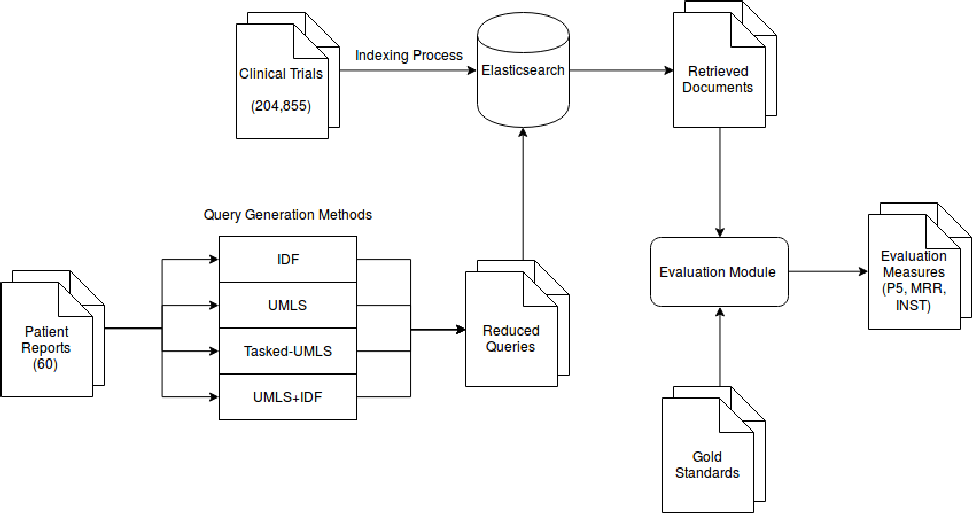
\includegraphics[width=1\columnwidth]{pipeline}
\label{eval-pipeline}
\end{figure}



% QUERY REDUCTION
\chapter{Query Reduction}
Query reduction is the process of taking an initial query and reducing it to a subset of its original terms via some pruning process. Balasubramanian et al.~\citep{Balasubramanian:2010:ERL:1835449.1835545} provide a formal definition of the query reduction task to find the set $P^*$:

\begin{equation}
\begin{split}
P^* &= \argmax_{P\in \mathcal{P}^Q} T_f(P),
\end{split}
\end{equation} where $Q$ is the original query, $\mathcal{P}^Q$ is the set of possible subqueries of $Q$, and $T_f$ is the measure of retrieval effectiveness for a given query. However, because it is not viable to calculate $T_f$ for every $P$, estimations must be made; this gives us the revised definition of $P^*$:

\begin{equation}
\label{QRdefinition}
\begin{split}
P^* &= \argmax_{P\in \mathcal{P}^Q} \widehat{T_f}(P)
\end{split}
\end{equation}

The query reduction task thus becomes the problem of finding an effective method of estimating values of $T_f$ in order to produce the best possible value of $P^*$.

\section{Methods}
\subsection{IDF-r Model}
One measure commonly used throughout the field of information retrieval is Inverse Document Frequency (idf). This is used to represent the importance of individual terms within the context of a given document collection. The idf of a particular term $t$ is calculated as follows:

$$idf_t = \log{\frac{1+N}{df_t}}$$
where $N$ is the total number of documents in the collection and $df_t$ is the document frequency of $t$ (number of documents in collection that contain $t$).

This method was used by Koopman et al.~\citep{koopman2017generating} to reduce a patient narrative to a subset of terms with the highest idf scores. Formally, a reduction resulting from this method can be seen as comprising of the terms in the following set:

$$Q' = \{ t : s(t,Q) \leq |Q| \cdot r \}$$
where $s(t,Q)$ is the ranked position of term $t$ within query $Q$ based on its idf score, $|Q|$ is the number of terms in the original query, and $r$ is the retention percentage.

\subsection{UMLS Model}
This model identifies and retains only those terms from the original patient narrative that form medical concepts. Medical concepts were identified as those belonging to the UMLS medical thesaurus. Medical terms were identified using QuickUMLS~\cite{Soldaini2016QuickumlsAF} - an information extraction system that maps free-text to UMLS concepts. This method has been used to reduce patient narratives both in context of clinical trials search, by Koopman et al.~\cite{koopman2017generating}, as well as clinical decision support, by Soldaini et al. \cite{Soldaini2015RetrievingML}; however, it has been reimplemented here for the purposes of comparison.

\subsection{Tasked-UMLS Model}
This is a variant of the UMLS model which applies a further layer of reduction to extract only those concepts that are classified as being \textit{Diagnosis}, \textit{Treatment}, or \textit{Test} related. This model was proposed by Koopman et al.~\citep{koopman2017generating} in light of prior studies showing that medical professionals typically pose clinical questions around these semantic types~\cite{Ely2000A-taxonomy-of-g}.

\subsection{UMLS+IDF-r Model}
The UMLS+IDF-r model is a combined approach proposed by Koopman et. al~\citep{koopman2017generating}, whereby the reduced query generated by the standard UMLS model is further reduced via the same protocol used by the IDF-r model. Formally:

$$Q' = \{ t : s(t,\mathbb{U}) \leq |\mathbb{U}| \cdot r \}$$

where $s(t,\mathbb{U})$ is the ranked position of term $t$ within the reduced query returned by the UMLS model $\mathbb{U}$ based on its idf score, $|\mathbb{U}|$ is the number of terms in the original query, and $r$ is the retention percentage.

\subsection{Health-Terms Model}
This query reduction model utilises a Wikipedia dump in order to calculate term weights. The official dump from 1/12/2016 was taken and filtered to contain only English language pages that were not talks, user pages or redirects, resulting in a collection of 9,195,439 pages. Each Wikipedia page has been classified as either \textit{health-related} or \textit{non-health-related} depending on whether or not their infobox contains one or more medical concepts as represented in the MeSH, UMLS, SNOMED CT, or ICD knowledge-bases. Query terms are then scored with the following formula:

\begin{equation}
\label{hrterms}
\begin{split}
OR(t) &= \frac{Pr\{ P \text{ is health-related } | t \in P\}}{Pr\{ P \text{ is not health-related } | t \in P\}}
\end{split}
\end{equation}
where $t$ is a term and $P$ is a Wikipedia page. A term is retained as part of the generated reduction if $OR(c_l) \geq \delta$, where $\delta$ is a tuning parameter. This method was tested with $\delta$ set to various different values in order to identify an optimal setting. 

\section{Experiment Settings}
We first analysed the change in retrieval effectiveness exhibited when the value of the threshold parameter $\delta$ changes. All patient narratives where subjected to the HT reduction process with $\delta$ being set to different values between 0.001-0.1 at steps of 0.001, and a search was executed for each of these reductions. This was done for both of the document corpora. Additionally, a similar analysis was performed with regard to the reduction proportion parameter, $r$, which is used by IDF-$r$ and UMLS+IDF-$r$. Here, 100 different settings of $r$ were tested for each model, from 0.01 to 1.0, in steps of 0.01.

The performance of all five query reduction models were tested within the context of each of the two corpora. For the Clinical Trials corpora, the evaluation measures P@5, MRR, and INST were used, with the results of the raw narratives, summaries, and human ad-hoc queries being used as baselines. For the Clinical Decision Support, the evaluation measures P@10, infAP, NDCG, and R-prec were used along with the raw narratives and summaries being used as baselines. 

\section{Results}

\subsection{Clinical Trials}

\begin{figure}
\centering
\caption{Reduction model comparisons for CT corpus.}
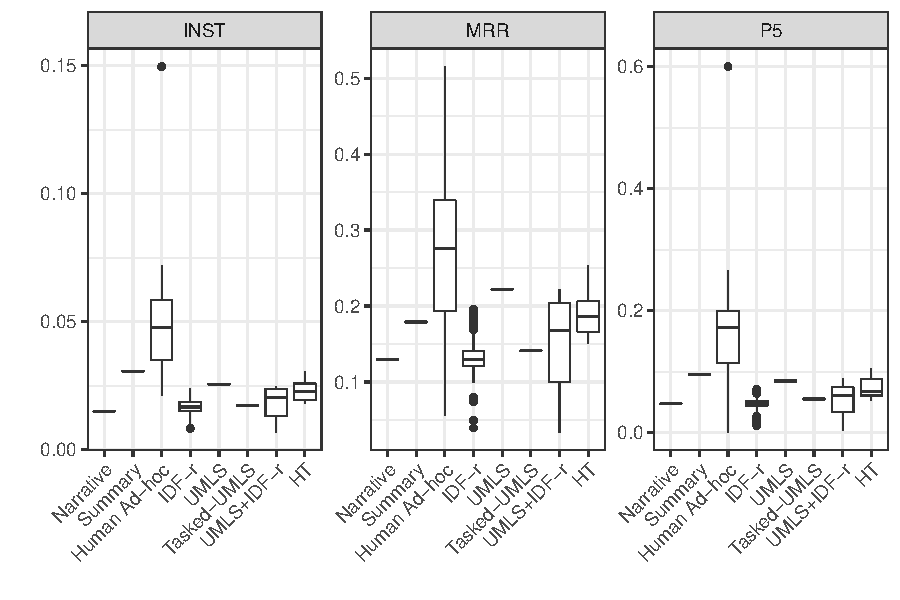
\includegraphics[width=.9\columnwidth]{ctreduction.pdf}
\label{fig:ct_results}
\end{figure}

A comparison of reduction model performances can be seen in Figure \ref{fig:ct_results}. The raw patient narrative appears to result in the poorest retrieval effectiveness, confirming the need for automated methods to be investigated. The summarised versions of these narratives seem to immediately show a noticeable improvement across all measures, suggesting that merely reducing the length of such verbose pieces of text results in improvement. Across all evaluation measures the human ad-hoc queries were clearly the most effective, with results outperforming all other methods to a statistically significant degree. This was to be expected, as these queries represent the ability of real life clinical experts. These ad-hoc queries not only represent a further degree of verbosity reduction over the narrative but are of a short keyword based format, which shows that although summarisation provides a potential for increased retrieval effectiveness, short keyword queries provide an even greater potential for improvement.

The IDF-$r$ reduction method appears to produce effective results for specific settings of $r$. In fact, when an appropriate setting for $r$ was selected, the model exhibited a significant increase in MRR over the raw patient narratives ($p=0.04$). It is important to note that the boxplot representing the IDF-$r$ method in Figure \ref{fig:ct_results} shows the mean results across all queries for each setting of $r$, many of which being highly sub-optimal. The figure includes results where $r$ is set to values between $0.01$ and $1.0$ in steps of $0.01$. For example, setting $r = 0.01$ (reducing the narrative to 1\% of its terms) would obviously not be an optimal reduction policy. A more detailed representation of the relationship between the value of $r$ and the model's retrieval effectiveness can be seen in Figure \ref{ct-idf-r}. This figure shows that for all three evaluation measures, performance increases with the value of $r$, eventually reaching a peak at around 0.25-0.30, before dropping in performance and eventually converging to the baseline level. Overall, the results for IDF-$r$ show that the removal of less informative terms is a simple, yet effective strategy for improving the retrieval effectiveness of patient narratives.

\begin{figure}
\centering
\caption{Query performance at different global settings of $r$.}
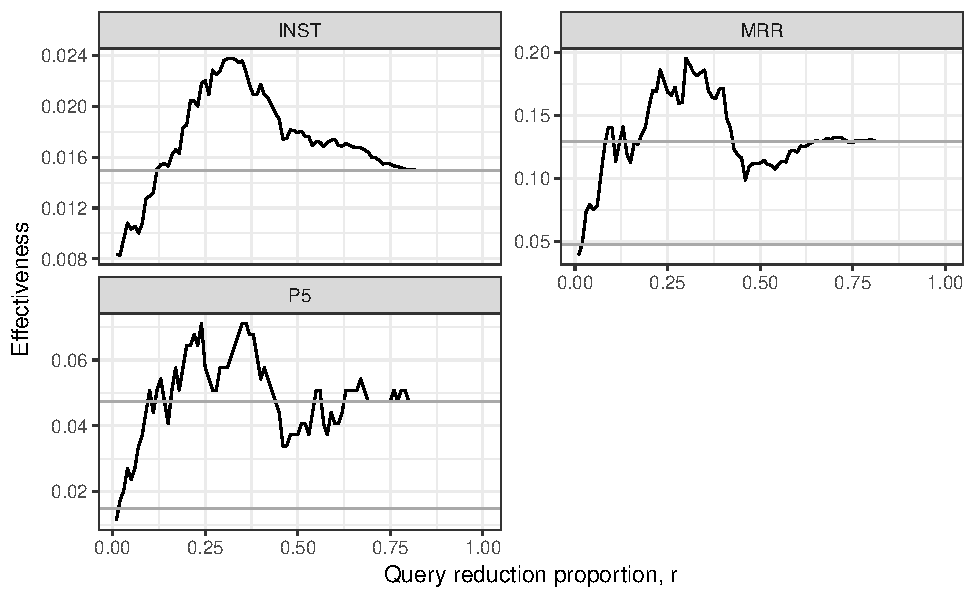
\includegraphics[width=.9\columnwidth]{ct-idf-r.pdf}
\label{ct-idf-r}
\end{figure}

The UMLS reduction method shows rather positive results. In terms of MRR this method showed significant improvement over using the raw narrative ($p = 0.031$), however did not show similar improvement over the narrative summaries ($p = 0.395$). Despite not being significant, it does clearly show some level of improvement over the summaries, suggesting that reducing patient narratives to contain only medical concepts is a relatively effective way to conduct searches. UMLS-based reductions also seem to produce better results than those of IDF-$r$, however this is not significant ($p = 0.088$). Tasked-UMLS proved to be a failure, yielding little to no improvement over the full patient narratives. This suggests that the extra layer of term reduction on top of the initial UMLS concept reduction is too aggressive.

The combined UMLS+IDF-$r$ method also appears to produce somewhat effective results when an appropriate setting of $r$ is selected. Note that the boxplot for UMLS+IDF-$r$ in Figure \ref{fig:ct_results} represents the same range of settings for $r$ as was used for IDF-$r$. However, the results for this model do not seem to be statistically significantly different from IDF-$r$ ($p = 0.072$) or UMLS ($p = 0.568$). Despite this, UMLS+IDF-$r$ managed to achieve similar retrieval effectiveness to these other two models with reduced queries containing far fewer terms.

The Health-Terms reduction method appears to produce the highest query effectiveness results of all automated methods when an optimal global setting of $\delta$ is selected. While its improvement over the raw narrative is significant ($p=0.075$), the same cannot be said for that over the summaries ($p=0.522$). The results in Figure \ref{fig:ct_results} also suggest that the Health-Terms model exhibits a prima facie greater level of consistency compared to the other variable-dependant models (IDF-$r$ and UMLS+IDF-$r$). However, it is difficult to say this with much level of certainty because, although the same number of different parameter settings have been tested, the relative scope of those settings are not totally comparable to one another given their rather different natures. A more in-depth representation of the relationship between the variation in retrieval performance and the value of $\delta$ can be seen in Figure \ref{fig:ctht_results}. This figure shows the MRR, INST and P@5 values for 100 different settings of $\delta$ between 0.001 and 0.1. From these results, it appears that the evaluation measures reach a peak when $\delta$ is set to a value of approximately 0.01 before gradually dropping in performance as this value grows.

\begin{figure}
\centering
\caption{Health-terms reduction effectiveness with differing values of $\delta$ for Clinical Trials corpus.}
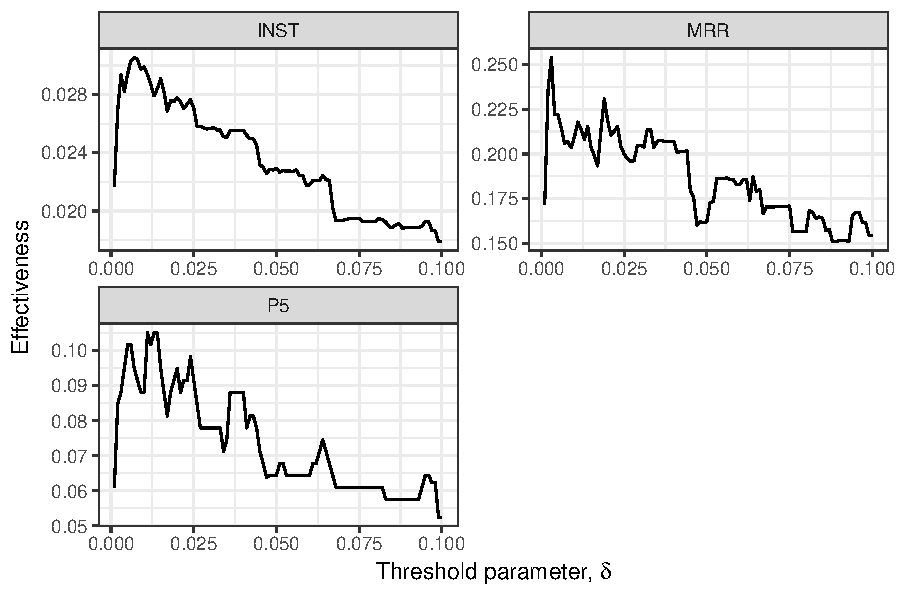
\includegraphics[width=.9\columnwidth]{cthtmodel.pdf}
\label{fig:ctht_results}
\end{figure}

An additional observation that can be made in relation to the human generated ad-hoc queries is their level volatility. The ad-hoc queries exhibited the greatest level of variation in effectiveness across all models. While all of the highest performing queries tested in the experiment were human generated, there are some that are amongst the worst performing queries across all models. A more in-depth investigation into the formulation of human generation queries and what factors contribute to their retrieval effectiveness would be useful in further understanding the cause of such volatility. One possible contributing factor can be identified after some initial analysis of the distribution of terms within these ad-hoc queries. It was found that 49\% of all human ad-hoc queries tested had a term overlap of 0.00 with their corresponding patient narrative; i.e the ad-hoc query had no common terms with the narrative, consisting entirely of novel terms introduced by the clinician. Furthermore, the average term overlap across all ad-hoc queries is only 0.26. What can be drawn from this is that human clinicians are much more inclined to formulate their search queries using their own inferred terms, rather than merely selecting the most important ones explicitly contained within the patient narrative. As a result of this human inclination to infer external information into their formulated query, it seems reasonable to suggest that automated methods consisting exclusively of a term reduction process may be handicapped by their inability to source terms outside the explicit scope of the narrative. 

\subsubsection{Query Reduction Proportion Prediction}

The results for both IDF-$r$ and UMLS+IDF-$r$ represent the average performance across all narratives when a global setting of the reduction proportion, $r$, is chosen. Due to there being a great deal of variation throughout the set of narratives, in terms of both length and content, choosing to enforce a global reduction proportion may have been rather sub-optimal. Thus, we investigated the effect of predicting $r$ on a per-query basis. 

The methodology taken here was influenced heavily by query performance prediction (QPP)~\citep{Kumaran2009Reducing-Long-Q}. A training set was constructed by generating a set of reduced queries, setting $r$ at different values between 0.01 and 1.0 in steps of 0.01. For each of these generated queries the following QPPs were calculated:

\textbf{Inverse Document Frequency (IDF):} This was calculated and
averaged across all query terms.
$$IDF_t = \log \frac{1+N}{df_t}$$  
where $N$ is the total number of documents in the collection and $df_t$ is the
document frequency of term $t$.

\textbf{SCQ:} A measure of how similar a query was to the collection as a
whole; averaged across all query terms. 
$$SCQ_w = (1+ \ln{\frac{n(w)}{N}}) \times \ln{(1 + \frac{N}{N_w})}$$
where $N_w$ is the document frequency of $w$, and $n(w)$ is the collection frequency of $w$. 

\textbf{Inverse Collection Term Frequency (ICTF):} This was calculated
and averaged across all terms. 
$$ICTF_w = \log_2{\frac{n(w)}{T}}$$
where $T$ is the total number of terms in the collection.

\textbf{Query Scope (QS):} A measure of the size of the retrieved document
set relative to the collection size: 
$$QS = -\log{\frac{n_Q}{N}}$$ 
where $n_Q$ is the number of documents that contain at least one of the query terms.

The correlation between these calculated QPPs and the retrieval effectiveness (on the basis of P@5) of each generated query was examined and the highest performing reduction(s) for each patient narrative was recorded. This resulted in a set of 1289 narrative, query pairs that were used as final training set for a Generalized Linear Regression Model. The training
data was stratified into four folds according to narrative id (60 narratives
divided into folds of 15 narratives). The model was trained to predict an optimal setting of $r$ for a given query from the calculated QPPs using 4-fold cross validation. The predicted settings of $r$ were subsequently used by IDF-$r$ and UMLS+IDF-$r$ and run through the evaluation pipeline. 

The results produced by this predictive component can be seen in Table \ref{tbl:glm}. It appears that using this model to predict $r$ on a per-query basis yields significant improvements to MRR over the global alternative; however, no significant changes to P@5 and INST can be seen. Table \ref{tbl:glm} also contains "oracle" results, which indicate the potential retrieval effectiveness in the case of a perfect prediction model. This was compiled by manually selecting the ideal setting of $r$ for each of the narratives. These oracle results showed a highly significant improvement over the case of a global $r$ setting across all three evaluation measures. Although these are merely the results of a hypothetical mode, they reveal to us that pure reduction techniques are capable of producing very high performing results when the narrative is reduced to the optimal degree. The considerable gap in performance between the implemented prediction model and the oracle results show that there is a great deal of room for improvement, and as such, an important area of future work would be in the development of a richer feature set for this predictive model. Particular points of inquiry would be in the evaluation of medical specific features, such as mentions of particular diseases affecting the patient, permanent demographic information (age, gender) and negated content (e.g. "no fever"). A more adept understanding as to what constitutes an effective human query would also help to inform such features.

\begin{table}
  \label{tbl:glm}
  \caption{Retrieval results when predicting query reduction proportion. Percentages show improvements and $\dagger$ show significance when compared to best global $r$.}
\begin{center}
  \begin{tabular}{@{}llll@{}}
    \toprule
    &P5&MRR&INST\\
    \midrule
    Human adhoc& 0.1521 & 0.2878 & 0.0476\\
    Narrative & 0.0508 & 0.1312 & 0.0149\\
    Summary & 0.0949 & 0.1790 & 0.0306 \\
    Average global $r$  & 0.0551 & 0.1513 & 0.0184\\
    Best global $r$ & 0.0881 & 0.2220 & 0.0247 \\
   Per-query $r$ --- QPP & 0.0861 (-2\%)  & 0.2432 (+10\%)$\dagger$ & 0.0268 (+9\%) \\
    Per-query $r$ --- Oracle & 0.1457 (+65\%)$\dagger$ & 0.3679 (+66\%)$\dagger$ & 0.0368 (+49\%)$\dagger$ \\
  \bottomrule
\end{tabular}
\end{center}
%\vspace{-16pt}
\end{table}



\subsection{Clinical Decision Support}
\begin{figure}
\centering
\caption{Reduction model comparisons for CDS corpus.}
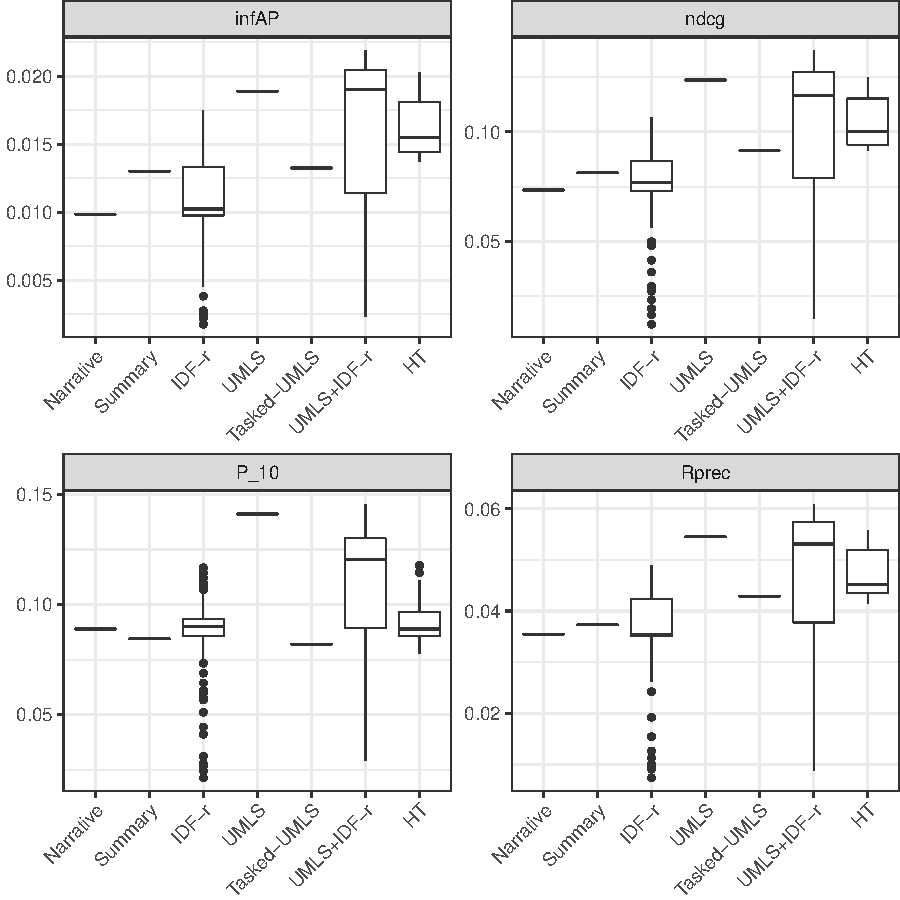
\includegraphics[width=.9\columnwidth]{cdsreduction.pdf}
\label{fig:cds_results}
\end{figure}

A comparison between the performance of all automated reduction methods, as well as the raw narrative and summary baselines, for each of the four evaluation measures (infAP, NDCG, P@10, R-Prec) can be seen in Figure \ref{fig:cds_results}. An initial observation shows that, similarly to the clinical trials, using the full patient narrative as a search query does not produce particularly desirable results. However, unlike the case of clinical trials, the summarised versions of these narratives do not appear to perform much better at all. In the case of P@10, the full narratives actually produce slightly more effective results than the summarised versions. 

IDF-$r$ once again appears to produce relatively good results when an optimal setting for $r$ is selected. In contrast to its performance in the context of the clinical trials documents, when an optimal setting of $r$ is chosen, the model appears to outperform the summarised patient narratives across all four evaluation measures. In terms of NDCG, this performance is significantly better than both the full narratives ($p=7.197e^{-06}$) and the summaries ($p=0.0199$). However, this could be more a result of poor performance on the part of the summaries as opposed to an improvement on the part of the IDF-$r$ model. The model continues to show a great deal of variation across different setting of $r$, however this is to be expected for the same reasons as were addressed in the previous section.

Once again, the UMLS reductions appear to be performing well across the board. In terms of NDCG, the UMLS reductions perform significantly better than the full narratives ($p = 1.315e^{-09}$), as well as the summaries ($p=2.154e^{-05}$). In addition to this, significant improvement is also seen when compared to IDF-$r$ at an optimal setting of $r$ ($p=0.02289$).

Tasked-UMLS seems to be performing at a similar level to what it is in the case of the CT collection. For NDCG, there is significant improvement over the full narratives ($p=0.02339$), but not over the summaries ($p=0.3065$). There is a notable drop in performance for every evaluation measure in comparison to the plain UMLS reductions ($p=0.0002$, for NDCG), reinforcing the idea that further restricting the the types of medical terms retained is consequently discarding important query concepts. In comparison to IDF-$r$ it also appears to be performing to the same level as what was seen for the CT collection, with IDF-$r$ performing better at optimal settings of $r$, however this is not significant ($p=0.1611$). 

The combined UMLS+IDF-$r$ method too shows similar comparative results to what was observed for the CT collection, however it now shows that, given an appropriate global setting of $r$, it is possible to achieve better results than the plain UMLS method, however this is not significant ($p=0.08834$).

The Health-Terms model performs significantly better than the full narratives ($p=1.111e^{-08}$) and summaries ($p=3.092e^{-05}$), at an optimal setting of $\delta$. However, it seems to exhibit worse performance in comparison to the other automated methods than can be seen within the context of the Clinical Trials collection. Here, the model  is observably outperformed by the UMLS ($p= 0.9249$) and UMLS+IDF-$r$ ($p=0.000142965$) reduction methods, even at optimal settings of $\delta$. However, the model still seems to significantly outperform both the IDF-$r$ ($p=0.02074$) and Tasked-UMLS ($p=0.001169$) methods. A more detailed breakdown of the relationship between $\delta$ and the retrieval performance can be seen in Figure \ref{fig:cdsht_results}. Similarly to what was observed with the Clinical Trials collection, all measures seem to quickly peak at approximately the $0.01$ mark before dropping off as this increases. However, this drop in performance seems to be much more dramatic than what was seen in the previous collection.

\begin{figure}
\centering
\caption{Health-terms reduction effectiveness with differing values of $\delta$ for CDS corpus.}
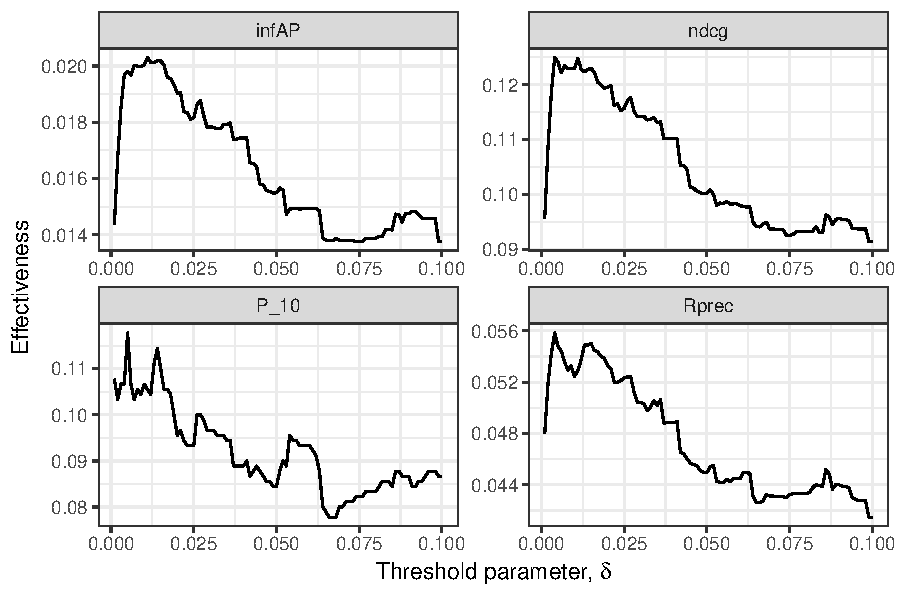
\includegraphics[width=.9\columnwidth]{cdshtmodel.pdf}
\label{fig:cdsht_results}
\end{figure}

Prior to further analysis into the nature of these results, it seems as though UMLS-based methods are performing better in comparison to the other methods in the context of the CDS collection, in addition to the summarised narratives performing worse. However, there are a few possible reasons as to why the situation may appear this way on its face. Firstly, a completely different set of evaluation measures to that used for the CT collection has been used here. Perhaps the observed differences between the models and baselines are tied to the nature of these new evaluation measures. In order to examine this further, the MRR and P@5 results for all models in the context of the CDS collection have been calculated and laid out in Figure \ref{cteval-cds}. However, these results do not in fact align with what was seen in the CT collection. In the case of the HT model, an even greater drop in performance is observed, relative to the other methods. In addition, the observed drop in performance for the summarised patient narratives when used to search the CDS collection still remains for these evaluation measures, with the full narratives actually performing slightly better than the summaries for both MRR and P@5. This clearly rules out the possibility of the performance differences merely being a result of using a different set of evaluation measures.

\begin{figure}
\centering
\caption{Model results for CDS corpus with evaluation measures of CT corpus.}
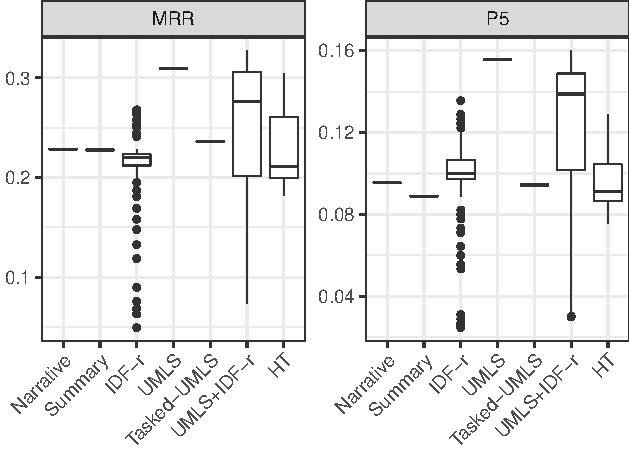
\includegraphics[width=.9\columnwidth]{reductioncompar.pdf}
\label{cteval-cds}
\end{figure}

The next obvious difference between the the two corpora which can be examined is the differing narrative sets. When testing the CT collection, 60 patient narratives were used, whereas in the case of the CDS collection, an additional 30 narratives were used on top of those 60. Perhaps these newly introduced patient narratives are the cause of the performance differences. In order to examine this, the evaluation results considering only those patient narratives shared with the CT collection have been computed and can be seen in Figure \ref{cdsreduction-1415}. These results look similar to what can be seen when all 90 narratives are considered, but for the summaries suddenly seeing a big performance increase, putting them closer to the relative position that they exhibit within the context of the CT corpus. This suggests that the poor performance previously observed for the summaries are a result of the 30 narratives unique to the CDS collection having poor summarised versions. Additionally, with optimal settings of $\delta$, the HT model now produces results closer to UMLS and optimally set UMLS+IDF-$r$. However, this is still below what is seen in the CT collection.

\begin{figure}
\centering
\caption{Reduction model comparisons for CDS corpus only considering patient narratives shared with CT corpus.}
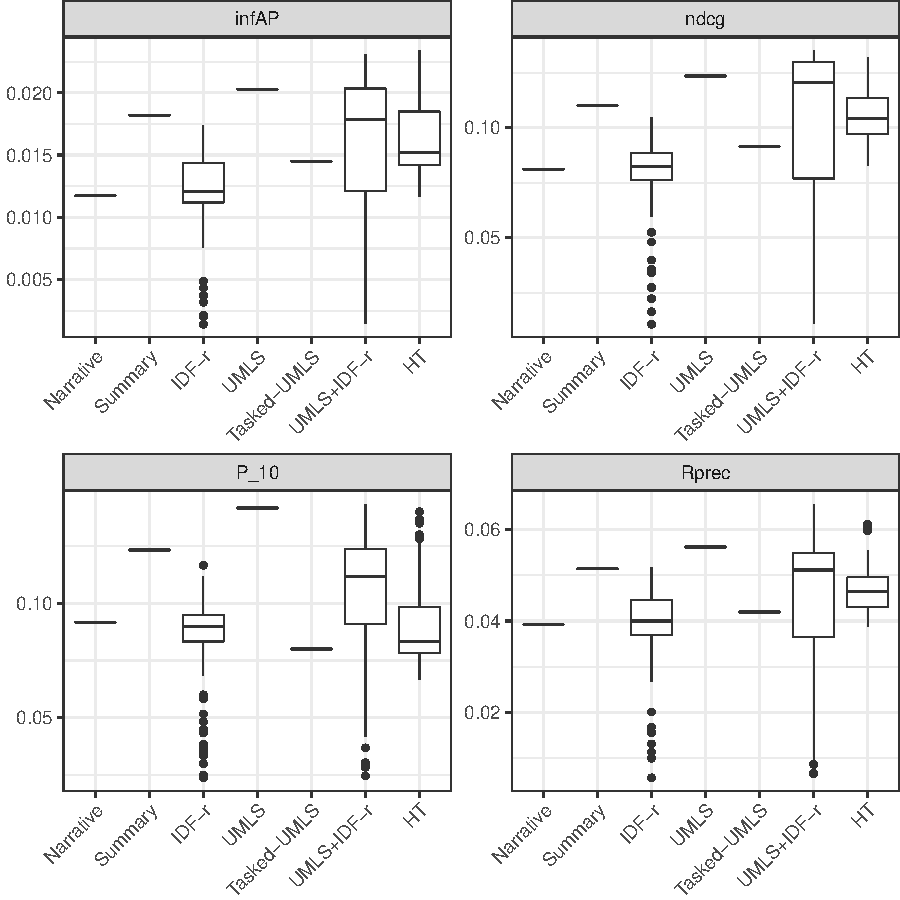
\includegraphics[width=.9\columnwidth]{cdsreduction-1415.pdf}
\label{cdsreduction-1415}
\end{figure}

This leaves us to consider what could be causing the relative drop in performance seen by the HT model when moving to the CDS corpus, in comparison to the UMLS-based methods. As both the UMLS and HT reduction processes are independent of the document corpus, the same set of reductions are being tested in both contexts. One possible explanation for this could be that the evaluation of retrieval results are being effected by the presence of unjudged documents. When the retrieval performance of a model is being evaluated, this is done by examining how many of the top documents are truly relevant in relation to the query. However, because document corpora are so large, generally only a limited number of documents are actually annotated as being \textit{relevant} or \textit{non-relevant}; these are known as \textit{judged documents}. For the remaining, \textit{unjudged} documents, it is unknown whether they are truly relevant or not and are generally treated as non-relevant in order to avoid overestimating the performance of a model. If a large number of top documents retrieved by the HT model are unjudged, this could result in a lower performance evaluation than what is truly being exhibited. 

In order to investigate the effect of unjudged documents the HT queries were first split into two classes: those that produced better retrieval results than their UMLS counterpart, and those that produced poorer results (on the basis of P@10). The number of unjudged documents residing within the set of the top 10 retrieved documents for each query was subsequently counted. These counts for each of the two corpora can be seen in Figure \ref{unjudged-boxplot}. In the case of clinical trials, the HT queries that perform better than their UMLS counterpart retrieve an average of 6 unjudged documents in their top 10 retrieved documents, and those that perform worse than their UMLS counterpart retrieve an average of 8. In the case of CDS, the higher performing HT queries retrieve an average of 4 unjudged documents, whereas the poorer ones retrieve an average of 5. This shows that the difference in the number of unjudged documents retrieved between the higher performing and lower performing HT queries remains uniform across the two collections in that the higher performing queries retrieve a smaller number of unjudged documents. The Clinical Trials collection also contains less judged documents than the CDS collection, so the higher number of unjudged documents retrieved is to be expected. Because of this, it remains unknown whether these poor performing queries are actually poor performing, or are retrieving documents that would otherwise be relevant, but for their unjudged status. The only way to truly shed light on how much of an effect these unjudged documents are having on performance evaluation would be to have these documents judged for relevancy in order identify the true performance of these reductions.

\begin{figure}
\centering
\caption{Avg. unjudged documents in top 10 retrieved by HT model.}
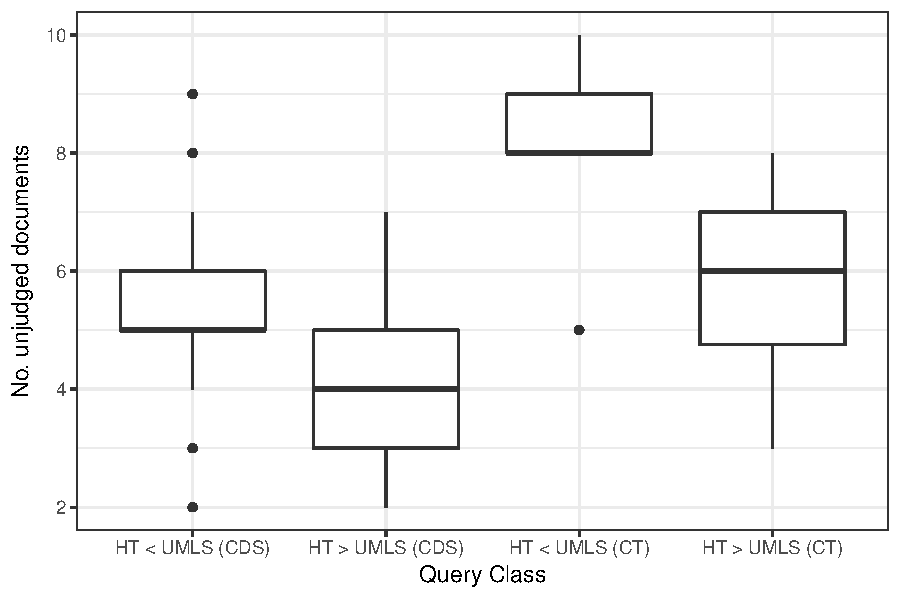
\includegraphics[width=.9\columnwidth]{unjudged-boxplot.pdf}
\label{unjudged-boxplot}
\end{figure}

Next, an investigation into reductions at the term level was conducted. Once again, the queries produced by HT were grouped into those that were higher performing and those that were worse performing than their UMLS counterpart. This was done in the context of both the document collections. From there, various statistics were calculated in order to form a more qualitative understanding of what is being produced by each of the two reduction methods.

The difference in query length between the two methods appears to stay relatively constant, regardless of the collection or level of performance. For the CT collection, higher performing HT queries were on average 5 terms shorter than their UMLS counterpart, and the poorer performing were on average 7 terms shorter. In the case of the CDS collection, the HT queries were on average 6 terms shorter than their UMLS counterpart, regardless of whether they were higher or poorer performing.

For the Clinical Trials collection, there appears to be a correlation between high idf and query performance. The higher performing HT queries yield an average idf of $4.4$, whereas the poorer performing queries yield an average idf of $3.9$. This is also seen in the case of the UMLS queries, with those performing better than their HT counterpart yielding an average idf of $3.545$ and those with a worse performance yielding $2.889$. This not only suggests that queries with idf-rich terms perform better, but also that the terms retained by the HT method have higher idf values.

However, these findings are not corroborated within the CDS collection. In fact, the higher performing HT queries actually yielded a lower average idf score ($4.293$) than the lower performing ones ($5.027$). The poorer performing UMLS queries also yield a higher average idf than the higher performing ones, but this is only by a very small margin ($4.363$ and $4.302$, respectively). It remains unclear as to why this might be occurring.

Next, a more qualitative approach was taken to examine what kind of terms were being retained by each of the two methods. All terms being retained exclusively by either HT or UMLS were grouped together and ranked based on \textit{tf*idf}. This is a common metric used in information retrieval to quantify how informative a particular term is with respect to a particular document and the document corpus at large. For the purposes of this particular experiment, this metric was calculated as follows:

$$\text{\textit{tf*idf}}(t) = freq(t)\cdot idf(t)$$

where $freq(t)$ is the number of times term $t$ is retained by the method across all of the patient narratives, and $idf(t)$ is the idf of $t$ with respect to the document corpus in question. 

The top 15 terms being retained by each of the two methods, in the context of either document corpus can be seen in Table \ref{retained-terms}. It appears as though across both corpora, the HT method seems to retain terms that are, on their face, more domain specific. The UMLS method does retain terms that could obviously be seen as having importance within a medical context, however they much more general and could be used throughout a wider range of context. The HT terms are much more specific to the domain and include some words that would presumably have no use outside of a medical context. Perhaps in the context of the CT collection, these more medically-oriented terms provide additional information that helps define the query scope more effectively, while potentially over-fitting to certain documents in the CDS collection. Perhaps where the more general terms retained by UMLS might be adding noise to the query in the context of the CT collection, they are helping to provide a more apt description of certain concepts with respect to the CDS collection. In order to further examine the effect here, a similar analysis could be conducted for not just individual terms but bi-grams and tri-grams. 

\begin{table}
\caption{Top 15 terms retained exclusively by HT or UMLS method.}
\label{retained-terms}
\begin{center}
  \begin{tabular}{|p{2cm}|p{5cm}|p{5cm}|}
  	\hline
      & \textbf{HT} & \textbf{UMLS}\\
     \hline
    ClinicalTrials & presents, hg, 9060, bp, nuclei, progressively, mildly, muffled, ellipsoidal, septated, markedly, bibasilar, radiates, normocytic, outstretched & complains, right, reports, pale, sounds, trip, left, productive, walking, history, family, tender, strawberry, admission, report\\
    \hline
    CDS & presents, hg, 9060, bp, mildly, hb, upper, muffled, 20ml, onset, mmhg, bibasilar, icu, radiates, progressively & history, complains, right, pale, sounds, walking, left, reports, admission, count, tender, day, heart, family, x-ray \\
    \hline
  \end{tabular}
\end{center}
\end{table}


% QUERY EXPANSION
\chapter{Query Expansion}
Despite seeing that automated query reduction techniques are able to improve retrieval effectiveness when applied effectively, this is fundamentally limited in that those techniques are only able to leverage terms and concepts that are explicitly included within the original query. However, human queriers infer and include many novel terms in their queries, which generally achieve a higher level of performance than pure reductions \citep{koopman2017generating}. Query expansion seeks to overcome this gap by making use of techniques that attempt to enhance a generated query by including new terms that are deemed to be relevant to the search task.

One popular query expansion technique used throughout information retrieval is pseudo-relevance feedback (PRF). PRF seeks to improve a query by adding a subset of the most informative terms existing within the top documents retrieved for that query. This acts on the assumption that the top documents are truly relevant, and by adding terms that are representative of those documents to the query, additional documents similar to those will hopefully be retrieved.

\section{Methods}
\subsection{Kullback-Leibler Divergence PRF Model}
Kullback-Leibler Divergence has been used as a scoring metric in PRF in an attempt to mitigate the problem of a term's score reflecting its importance with respect to the entire collection more than its importance with respect to the query itself~\citep{Carpineto:2012:SAQ:2071389.2071390}. It does this by taking into account the difference in term distribution between the set of pseudo-relevant documents and the entire document corpus. The Kullback-Leibler formula used to score expansion term candidates is as follows:

\begin{equation}
\label{kld-feedback}
\begin{split}
p(t|R) \cdot \log{\frac{p(t|R)}{p(t|C)}},
\end{split}
\end{equation}
where $p(t|R)$ and $p(t|C)$ are the probability of term $t$ occurring in the set of pseudo-relevant documents $R$ and entire document collection $C$, respectively.

Formally, the expanded query can be defined as:

$$Q' = Q \cup \{ t \in \mathbb{C} : r(t,\mathbb{C}) \leq j \}$$
where $Q$ is the original query, $t$ is a term in the candidate set $\mathbb{C}$, $r(t,\mathbb{C})$ is the ranked position of $t$ in $\mathbb{C}$ according the the KLD function, and $j$ is the number of terms to add.

\subsection{Rocchio PRF Model}
The Rocchio relevance feedback algorithm adopts a vector space model that attempts to maximise the difference between the average vector representing the set of relevant documents and the average vector representing the non-relevant documents \cite{10020859664}. It does so by modifying the query term weights by adding a component based on the average weight in the relevant documents and subtracting a component based on the average weight in the non-relevant documents. The Rocchio term weighting function commonly takes the following form \cite{croft2010search}:

\begin{equation}
\label{rocchioalg}
\begin{split}
  q'_j &= \alpha \cdot q_j + \beta \cdot \frac{1}{|Rel|} \sum_{D_i\in Rel} d_{ij} - \gamma \cdot \frac{1}{|Nonrel|} \sum_{D_i \in Nonrel} d_{ij} 
\end{split}
\end{equation}
where $q_j$ is the initial weight of query term $j$, $Rel$ is the set of identified relevant documents, $Nonrel$ is the set of non-relevant documents, $d_{ij}$ is the weight of the $j$th term in document $i$, and $\alpha$, $\beta$, and $\gamma$ are parameters that control the effect of each component. As a result of this weighting scheme, the query is not only modified through the addition of new terms, but by each query term being weighted by a boost coefficient. 

Soldaini et al.~\cite{Soldaini2015RetrievingML} adopted a version of this approach in the context of CDS search, which has been followed as a guide for the implementation used in the following experiments. The initial query is expanded by building the root set $\mathcal{R}_Q$, which consists of all terms appearing in either the query $Q$ or one of the top-$k$ documents retrieved by $Q$. The boost coefficient $b_m$ is then calculated for $t_m \in \mathcal{R}_Q$ as: $$b_m = \log_{10}(10+w_m)$$
where 
\begin{equation}
\label{prfscore}
\begin{split}
  w_m &= \alpha \cdot I_Q(t_m) \cdot tf_m + \beta/k \sum^{k}_{i=1} I_{D_i}(t_m)\cdot idf_m
\end{split}
\end{equation}
and where $I_Q(t_m)$ is an indicator of the presence of term $t_m$ in $Q$; $I_{D_i}(t_m)$ is an indicator of the presence of term $t_m$ in the document $D_i$; $idf_m$ is the inverse document frequency of the $m$-th term in the top $k$ documents; and $\alpha$ and $\beta$ are smoothing factors. Once all weights have been calculated, the terms in $\mathcal{R}_Q$ are ranked by their boost coefficient and the top $j$ terms not appearing in $Q$ are added to the query. When the search is initiated for the expanded query, every term is weighted by their boost coefficient, $b_m$. The following values were used for the smoothing factors throughout the experiment: $\alpha = 2$, $\beta = 0.75$.

\subsection{Health-Terms PRF Model}
The Health-Term PRF model operates in a similar fashion to that of the KLD-based model, but uses the health-relatedness score outlined in Equation \ref{hrterms} as the term scoring function. The set of non-query terms contained within the top-$k$ retrieved documents are extracted, applied to this function, and reduced to the top-$j$ terms according to this score. These terms are promptly added to the initial query in order to construct a new, expanded query.

\subsection{Health-Terms+Rocchio PRF Model}
This model is influenced by the \textit{HT+PRF} model proposed by Soldaini et al.~\cite{Soldaini2015RetrievingML}. It acts as a combination of the Rocchio and Health-Term PRF models, whereby the Rocchio weights are calculated for all candidate terms; however, instead of expanding the initial query with the top-$j$ terms, the expanded query is constructed by including all candidate terms with a health-relatedness score exceeding some threshold value, $\delta$. As a result, the number of terms added to create the expanded query is potentially different for every query. Formally, the expanded query $Q'$ can be defined as:

$$Q' = Q \cup \{ t \in \mathbb{C} : h(t) \geq \delta\}$$
where $Q$ is the original query, $t$ is a term in the candidate set $\mathbb{C}$, $h(t)$ is the health-relatedness score of $t$, and $\delta$ is the threshold parameter. Just like in the Rocchio model, all terms in $Q'$ are weighted by their boost coefficient, $b_j$.

\section{Experiment Settings}
We experimented with the performance of these methods within the context of the clinical trials document collection. PRF functionality was applied to the existing UMLS reduction model in order to identify additional terms that may be relevant, given the retrieval results of the UMLS reduced queries. Experiments were run with the number of pseudo-documents $k$ set to 3, 5, 7, and 9, and, for each of these, the number of pseudo-relevant expansion terms $j$ was set to values between 1 and 15, in increments of 2. In the case of Health-Terms+Rocchio, the threshold parameter $\delta$ was modified in place of $j$, at values between $0.25$ and $2.0$, in steps of 0.25.

\section{Results}

\subsection{Clinical Trials}
The retrieval performance with respect to parameter tuning can be seen in figures \ref{kldprf_results}, \ref{htprf_results}, \ref{rocchioprf_results}, and \ref{rocchiohtprf_results}. What can be seen generally across most models and setting of $k$ is that some improvement is seen initially, but as the value of $j$ increases, the performance begins to drop off. This is to be expected, as what is likely happening here is that less informative terms that may not be directly relevant within the context of the query are being introduced. This will naturally result in query-drift whereby the new query formulation will no longer reliably represent the meaning of the query, but rather become a reflection of the pseudo-relevant document set. 

A general trend can also been seen between values of $k$ in that performance starts to improve as $k$ increases from 3, but then starts to drop again as it reaches $9$. This shows us that using a smaller set of pseudo-relevant document to derive term scores from limits how informative those scores can actually be. By capturing a larger set of pseudo-relevant documents, it allows us to derive those term scores from a larger sample and thus resulting in more accurate, representative scoring functions. However, as $k$ exceeds more than approximately 5 to 7, this reliability of term scores once again drops. What is likely occurring here is that set of pseudo-relevant documents are starting to include many documents that are not truly relevant to the initial query, which subsequently contaminates the term scoring function. This, combined with a large value of $j$, naturally produces a notable drop in performance as a result of significant query drift.

In regards to the INST evaluation measure, consistent improvement over the baseline can be seen across all tested PRF models. This follows the general trend of reaching peak performance with $k$ and $j$ at values around 5 to 7, before dropping off again. 

In contrast to this, little to no improvement can be seen for P@5 and MRR across the board. This is likely resulting from the definition of these two evaluation measures. In the case of P@5, what is being measured is the proportion of the top 5 retrieved documents that are deemed to be relevant. As an example scenario, consider the case where the top 2 documents are in fact relevant, but the remainder of the top 5 are not. As soon as the PRF algorithm uses a value of $k = 5$ the majority of the pseudo-relevant document set is in fact non-relevant. This will result in an unrepresentative term scoring function whereby the top 2 documents will quickly start to drop in ranking. In the case where the top retrieved documents are not relevant to begin with, then query drift will start to be exhibited immediately with no real chance of improvement in performance. Essentially, the degree of possible improvement is fundamentally limited in that the only the top 5 documents are even being considered in order to derive the performance measure, and a term scoring that is seeded predominately by these documents will only serve to reaffirm their ranking.

A similar situation is probably occurring in the context of MRR. This measure considers the rank position of the first relevant document in the retrieved set. As has been mentioned above, the rank order of the top documents is not likely to change due to the self-affirming nature of the PRF term scoring function. Even in a situation where additional relevant documents are moved up in the rankings, only the position of the first relevant document is considered by the evaluation measure.

However, many of these observations do not apply to Health-Terms+Rocchio which exhibits results much different to what is seen in the other three models. Health-Terms+Rocchio shows an ability to improve over the baseline for all three tested evaluation measures. Changing the value of $k$ doesn't appear to have a drastic or even notable effect upon these results, with all settings following very similar trends. In regards to the threshold parameter, $\delta$, results are rather poor for smaller settings but begin to climb as this increases before seemingly starting to approach convergence as this value gets to around the $2.0$ mark. This is to be expected, as rather than expanding the query with a larger set of terms like what is seen with $j$, this parameter limits the number of terms that added. Furthermore the number of terms added is not fixed, it is based on whether or not their \textit{health-relatedness} is above $\delta$, which means that the number of expansion terms  has the potential to be completely different across the set of queries. This can arguably be seen as an overall better policy for expansion term selection, as terms that may not be helpful aren't added merely for the purpose of satisfying an arbitrary quota. An additional factor that differentiates this model from the other three is that not only does it expand the initial query with new terms, it applies a boost coefficient to all terms comprising the query (new and existing). This introduces a further layer of query adjustment that is not possible with the other models. 

\begin{figure}
\centering
\caption{Results for Kullback-Leibler Divergence PRF model.}
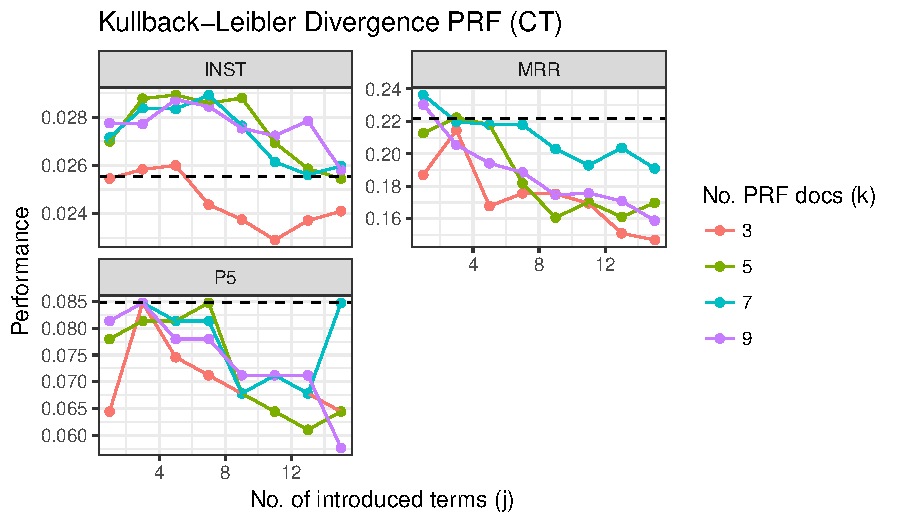
\includegraphics[width=.9\columnwidth]{kldprf.pdf}
\label{htprf_results}
\end{figure}

\begin{figure}
\centering
\caption{Results for Health-Terms PRF model.}
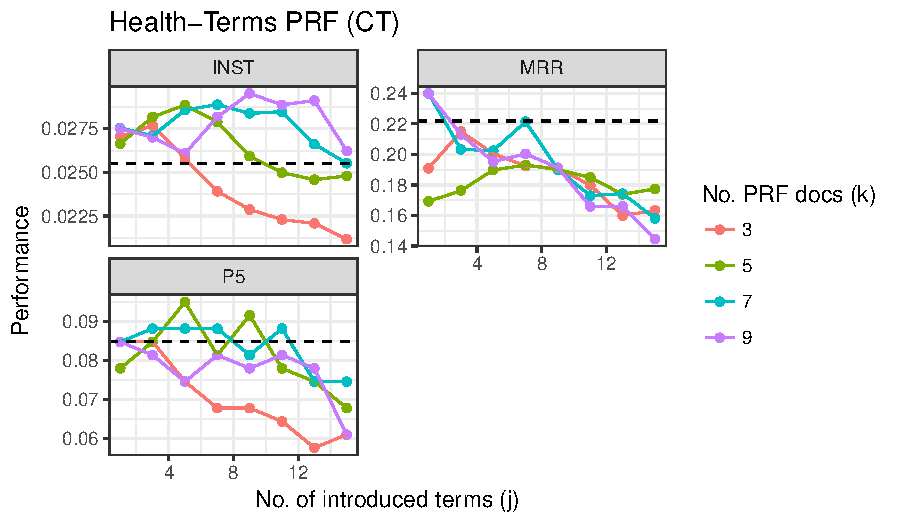
\includegraphics[width=.9\columnwidth]{htprf.pdf}
\label{htprf_results}
\end{figure}

\begin{figure}
\centering
\caption{Results for Rocchio PRF model.}
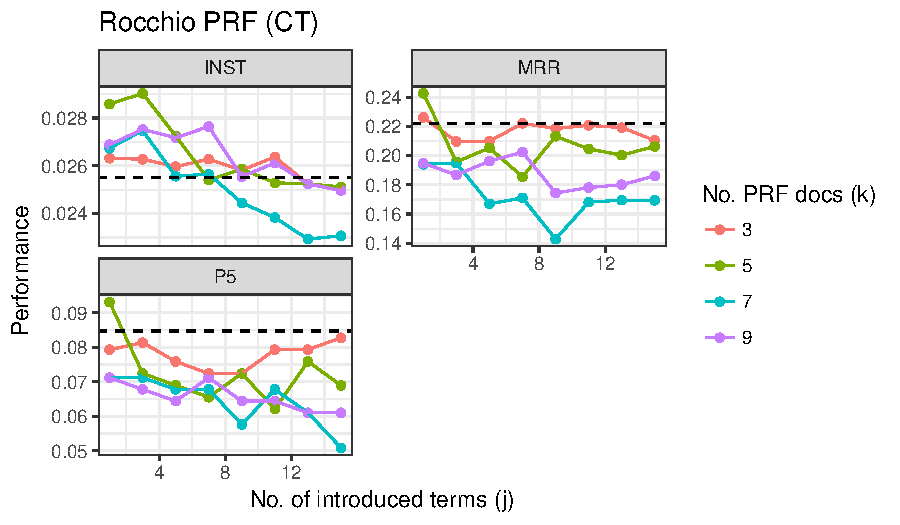
\includegraphics[width=.9\columnwidth]{rocchioprf.pdf}
\label{rocchioprf_results}
\end{figure}

\begin{figure}
\centering
\caption{Results for Health-Terms+Rocchio PRF model.}
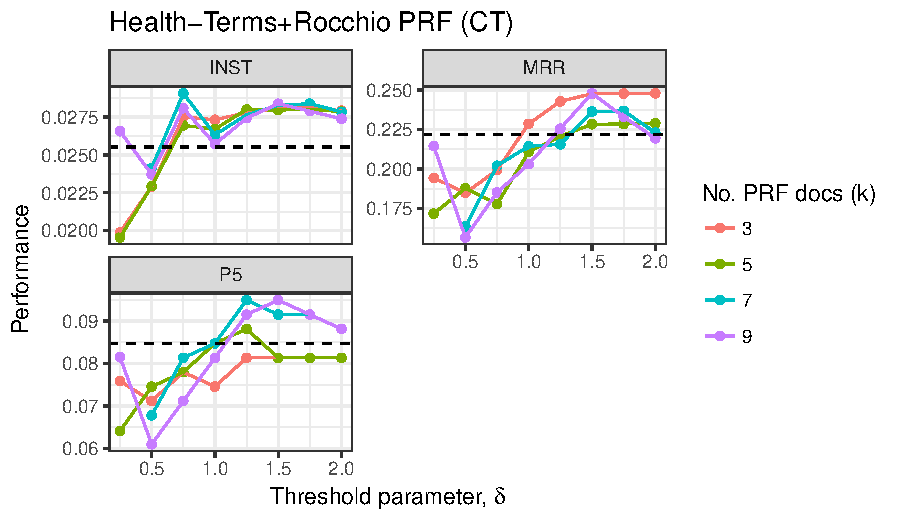
\includegraphics[width=.9\columnwidth]{ct-rocchiohtprf.pdf}
\label{rocchiohtprf_results}
\end{figure}

\begin{figure}
\centering
\caption{All query generation results for CT collection.}
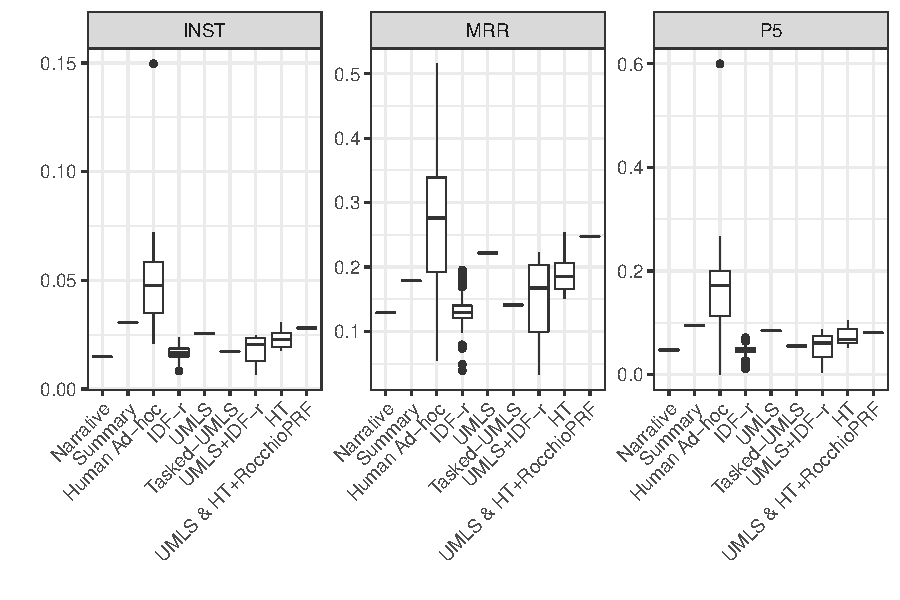
\includegraphics[width=.9\columnwidth]{ct-generation.pdf}
\label{ct-total}
\end{figure}


\subsection{Clinical Decision Support}
The same set of PRF methods were tested in the context of the Clinical Decision Support collection. The same range of experiments were conducted, with $k=1$ to $9$ and $j = 1$ to $15$. The general performance trends observed here are rather different to what can be seen in the CT results. On its face, there appears to be notably more potential for performance improvements as a result of using PRF in the case of the CDS collection. The degree of performance increase seen in the case of P@10 across the three PRF methods is rather limited and varied, however the other three evaluation measures showed considerable improvements over the baseline with optimal parameter settings.

The Kullback-Leibler Divergence PRF method produced fairly consistent levels of performance increase across all measures, with a peak being achieved when $j$ is set to approximately 3. However, instead of subsequently dropping in performance as this value increases, the performance level appears to remain relatively constant from this point onwards. Additionally, the optimal setting of $k$ appears to be 3, which is another feature that differs from what was seen with the CT collection. However, this may be a result of the different set of evaluation measures used with this collection. Also, the general trend is not followed in regards to P@10 here, which shows a decline  in performance as $j$ increases; however, $k = 3$ continues to be optimal here. With an optimal setting of $k$ and $j$, this method produces a NDCG score that is significantly better than that of the UMLS reduction method ($p=0.00685$).

\begin{figure}
\centering
\caption{CDS results for KLD PRF model.}
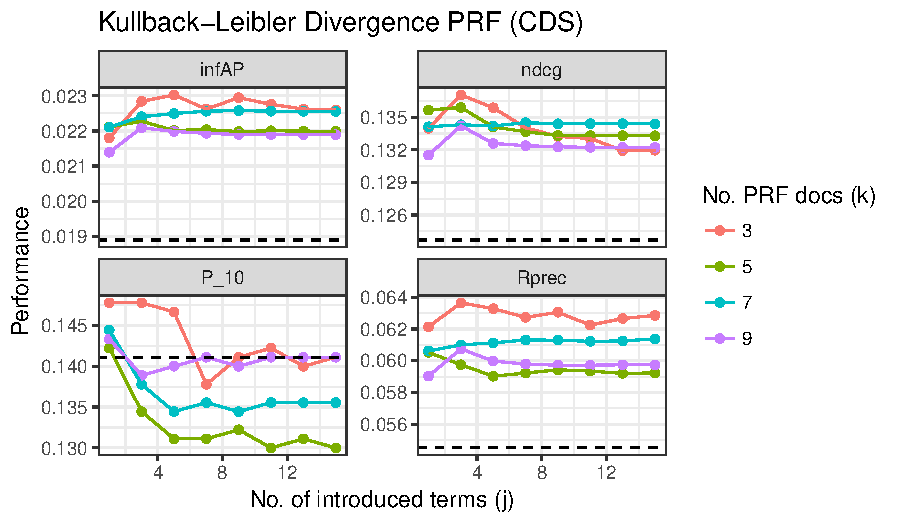
\includegraphics[width=.9\columnwidth]{cds-kldprf.pdf}
\label{cds_kldprf_results}
\end{figure}

The Health-Terms PRF method yields similar performance trends to the KLD method, but with greater variance across the different parameter settings. When $k$ is set to 3 or 5, some minor increase over the baseline in terms of infAP, NDCG and R-Prec can be seen, however higher settings of $k$ shows little to no improvement over the baseline. At optimal settings of $k$ and $j$ this method is still able to produce NDCG results that are better than the standard UMLS method, however this is not significant ($p=0.5163$). In the case of P@10, no improvement over the baseline is seen for any of the parameter settings. In fact, any increase in the value of $k$ or $j$ appears to correlate with a general drop in performance. Even at optimal parameter settings, this method is clearly outclassed by the KLD method, both in regards to potential performance gain ($p=0.03102$), and consistency. 

\begin{figure}
\centering
\caption{CDS results for Health-Terms PRF model.}
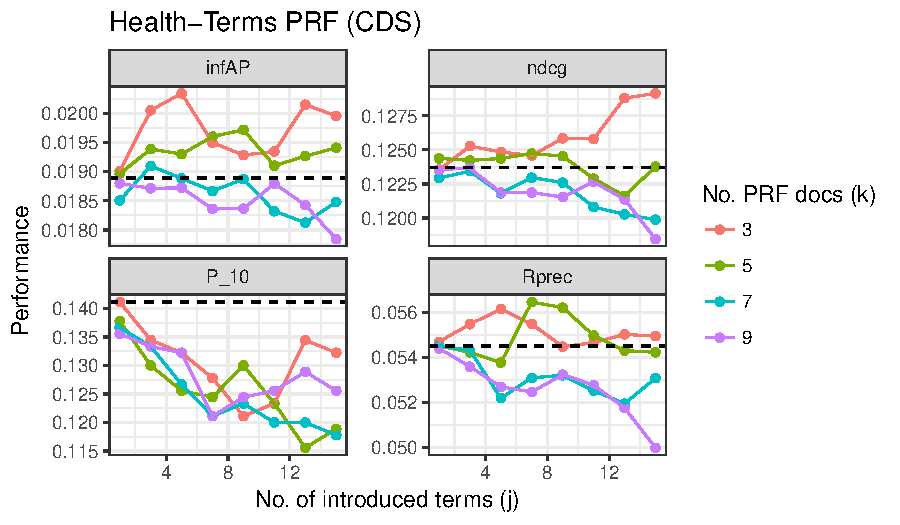
\includegraphics[width=.9\columnwidth]{cds-htprf.pdf}
\label{cds_htprf_results}
\end{figure}

The Rocchio method appears to produce results following a similar trend to what is seen for the KLD approach; however, where the KLD method converges at a particular level of performance gain, the Rocchio method continues to improve ($p=2.645e^{-05}$ with both models at optimal settings). In the case of infAP, NDCG and R-Prec, performance gain appears to gradually improve as $j$ increases. The optimal setting of $k$ for these three measures is 7, with maximal performance gain (observed within this range of tests) being reached where $k=7$ and $j=11$. Even in the case of P@10, the Rocchio method shows reasonable improvement over the baseline when $k>3$, reaching a peak when $k=5$ and $j=5$. This method was clearly produced the greatest performance gain over the baseline out of all of the PRF models. At optimal settings of $k$ and $j$, this method produces a NDCG score that is significantly better than that of the UMLS reduction method ($p=2.456e^{-05}$). 

\begin{figure}
\centering
\caption{CDS results for Rocchio PRF model.}
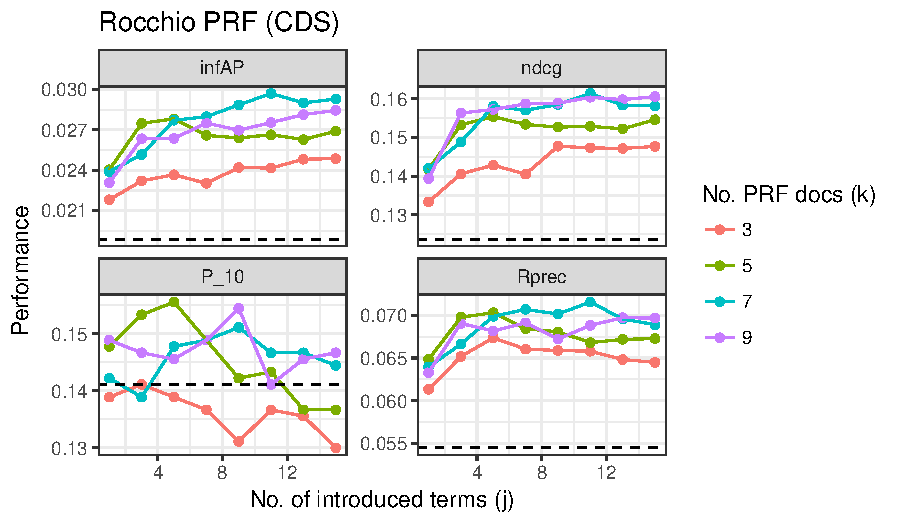
\includegraphics[width=.9\columnwidth]{cds-rocchioprf.pdf}
\label{cds_rocchioprf_results}
\end{figure}

In contrast to the CT collection, the Health-Terms+Rocchio model did not produce particularly good results. The degree of performance gain possible with this model appears to be rather conservative, showing very minor improvements over the baseline and, in the case of P@10, almost no potentiality for improvement. The results exhibited by this model are rather similar, in both performance level and internal trends, to those of Health-Terms. This is not particularly surprising, considering that both of their term selection policies are heavily structured around the \textit{health-relatedness} metric. Both of the models appear to observe a general decrease in performance with the increase of $k$, with the results of the half of tests with lower settings of this parameter and the half with higher settings appearing to diverge from each other with the increase of $j$, or conversely, the decrease of $\delta$. 

This observation reveals what may be one of the biggest downsides to the threshold oriented term selection policy utilised by the Health-Terms+Rocchio model. By basing candidate term approval on the value of a metric, without controlling the size of the approved set, the floodgates are opened to a potential influx of a large number of unhelpful terms. In particular, when $k$ is set to a high value, in many cases, a large proportion of those top-$k$ documents are not relevant to the query. By then only basing expansion term selection on the term's \textit{health-relatedness} metric, many terms that, while potentially being convincingly health-related, are from a document that has no relevance to the search query will still be added to the expanded query. This creates a query-drift-like effect, similar to what has been discussed with regard to the other models, but without the safety-net inherent in a model that only expands the query with an exhaustive number of new terms. Additionally, the relatively poor performance of both the Health-Terms and Health-Terms+Rocchio models here reaffirm the idea that the \textit{health-relatedness} metric is less powerful in the context of the CDS corpus than what can be observe in the case of the CT corpus.

\begin{figure}
\centering
\caption{CDS results for Health-Terms+Rocchio PRF model.}
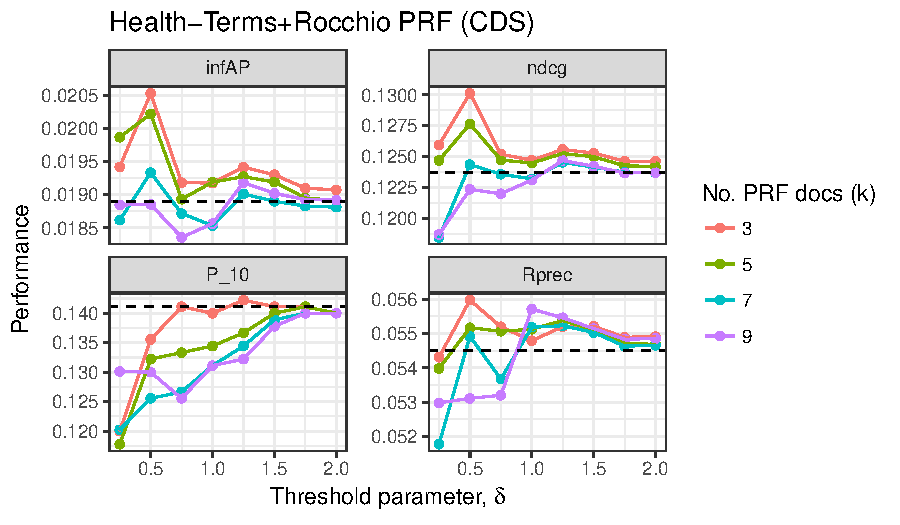
\includegraphics[width=.9\columnwidth]{cds-rocchiohtprf.pdf}
\label{cds_rocchiohtprf_results}
\end{figure}


\begin{figure}
\centering
\caption{All query generation results for CDS collection.}
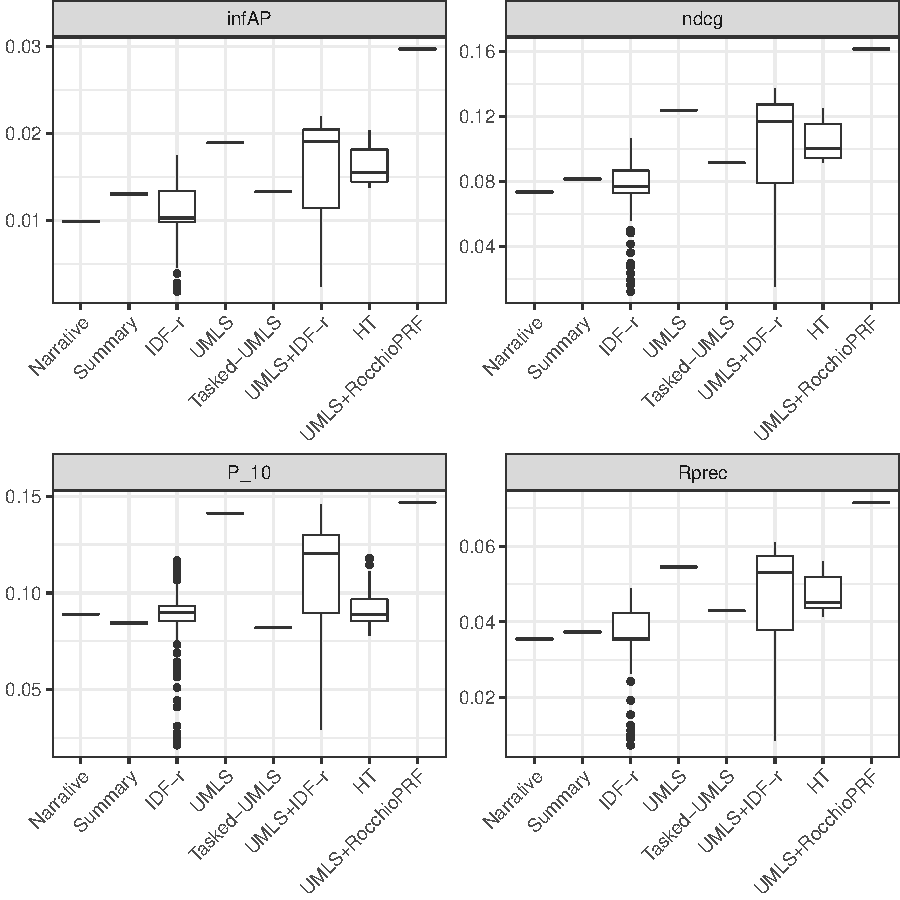
\includegraphics[width=.9\columnwidth]{cds-generation.pdf}
\label{cds-total}
\end{figure}

% CONCLUSION / DISCUSSION
\chapter{Conclusion}
\section{Summary}
In summary, this project has been successful in identifying effective automated query generation strategies for patient narratives. A range of query reduction methods that produce queries which perform significantly better than the full narratives have been identified. Although generally these do not perform as well as human formulated queries, under optimal conditions it has been shown that it is possible for some of these to produce queries that are competitive with those formed by humans. A predictive model that can effectively identify an optimal reduction proportion on a per-query basis could greatly improve the general performance of these reduction techniques. What constitutes an appropriate predictive model is yet to be determined.

In addition to this, various query expansion techniques that are capable of improving queries produced by the reduction techniques have been identified. At appropriate parameter settings, some of these methods are capable of significantly improving retrieval performance from what is produced by the pure reduction methods. In the context of Clinical Decision Support, PRF techniques exhibit an ability to produce very high results, with the Rocchio model in particular showing an improvement over the standard UMLS reduction method, with a p-value of $2.456e^{-05}$.

\section{Future Work}
There remains several avenues for future work arising from this project; particularly with regard to query generation methods examined in the literature review that were not directly investigated within the project. In terms of query reduction, one significant technique that was not investigated was the key-concept identification model proposed by Bendersky and Croft \cite{Bendersky:2008:DKC:1390334.1390419}. Furthermore, the performance of a concept-retrieval model, such as that proposed by Koopman et al.\cite{Koopman2011AEHRC--QUT-at-T} could also be subject to investigation. Additionally, the development of a richer feature set for the query performance prediction of clinical queries would make the task of predicting per-query reduction proportions more viable.

In regards to query expansion, this work only investigated pseudo-relevance feedback techniques. Although these methods showed some promise when it comes to retrieval performance gain, there are still a vast number of more complex techniques that could be examined within the context of this task. For instance, an implementation of a probabilistic graphical model for the purposes of term inference, similar to those seen in Koopman et al.\cite{Koopman2015Information-Ret} and Xue et al.\cite{Xue:2010:IVQ:1871437.1871572} could prove extremely valuable.

Finally, a more thorough investigation into human query formulation could prove helpful in assisting the development of novel term inference techniques, particularly in the clinical search domain. By forming a more in-depth understanding of what identification strategies human clinicians are exploiting when formulating their concise keyword-based queries, we would be able to more effectively utilise domain knowledge bases within automated techniques. 


\bibliographystyle{plain}
\bibliography{mybib}
\end{document}